\documentclass[10pt]{article}
\usepackage[margin=1.1in]{geometry}
\usepackage{amsmath,amssymb,amsthm}
\usepackage{booktabs}
\usepackage{multirow}
\usepackage{natbib}
\usepackage{microtype}
\usepackage[colorlinks=true,linkcolor=blue,citecolor=blue]{hyperref}
\usepackage{algorithm}
\usepackage{algpseudocode}
\usepackage{tikz}
\usetikzlibrary{arrows.meta,positioning,calc,decorations.pathreplacing}

% Custom Math Macros
\newcommand{\E}{\mathbb{E}}
\newcommand{\ind}[1]{\mathbf{1}\!\left[#1\right]}
\newcommand{\sg}{\mathrm{sg}}

\title{A Two-Phase Curriculum for Goal-Conditioned Visitation Values\\ from Manipulation Play Data}
\author{}
\date{}

\begin{document}
\maketitle


\section{Setting}

Offline data $\mathcal{D}$ of unlabeled ``play'' trajectories from OGBench \texttt{cube-single-play-v0} \citep{park2024ogbench} (state observations; a robot arm and one cube; $\sim$1M transitions).
The goal of the program is zero-shot RL in the sense of \citet{touati2021learning,touati2023does}: train once on $\mathcal{D}$ without rewards; at test time, given a reward function (specified by labeled samples), produce a policy with no further training.
The central object is the successor measure
\[
M^{\pi}(s,a,X) \;=\; \E_{\pi}\Big[\textstyle\sum_{t\ge 0}\gamma^{t}\,\ind{s_{t+1}\in X}\;\Big|\;s_{0}=s,\,a_{0}=a\Big],
\]
the discounted occupancy of state sets $X$ \citep{dayan1993improving,blier2021learning}.
Given $M^{\pi}$ for the right policies, any reward $r$ yields
$Q_r(s,a)=\int r\,dM^{\pi}(s,a,\cdot)$, hence zero-shot evaluation and (with a policy-improvement step) zero-shot control.
FB representations \citep{touati2021learning} learn a factorization
\[
M^{\pi_z}(s,a,X) \approx \int_X F(s,a,z)^{\top}B(x)\,dx,
\]
in which the \emph{policy index} $z$ and the \emph{queried future state} $x$ are separate
arguments: one fixed continuation policy $\pi_z$, occupancy of every $x$ under it.

\textbf{Scope of this note.} What we train below is not yet this full object.
It is the \emph{diagonal slice} $g \mapsto M^{\pi_g}(s,a,B_\epsilon(g))$ --- the visitation
value of a goal region under that goal's own policy (Section~\ref{sec:object}).
This suffices for goal-reaching tasks and for composition over small candidate-goal sets,
and it is where the training-stability content of the note lives; extending it to the
separated $(z,x)$ form needed for arbitrary rewards is ongoing work
(Section~\ref{sec:dense}).

\paragraph{The problem.}
On this domain, methods built on future-state reachability --- FB, successor features, contrastive value functions --- sit far below goal-conditioned TD baselines trained on the same data with the same actor class: FB variants plateau around $0.42$ overall success while goal-conditioned IQL \citep{kostrikov2021offline} with a bilinear critic reaches $0.90$.
The gap is not exploration or data: everything is offline and shared.
Something about the successor-measure \emph{objective} fails here.

\section{What the goal-conditioned baseline gets right}
\label{sec:baseline}

The strongest method on this data is not a successor-measure method at all: goal-conditioned
IQL with a \emph{bilinear} critic $Q(s,a,g)=\phi(s,a)^{\top}\psi(g)/\sqrt{d}$, trained by
expectile TD on the sparse $0/{-1}$ goal-reaching reward with hindsight-relabeled goals,
reaches $0.904$.
This baseline settles two questions before we change anything:

\begin{enumerate}
  \item \textbf{The factored representation is not the bottleneck.}
  The bilinear critic \emph{is} the rank-$d$ factorization that successor-measure methods
  use: $\psi(g)$ is a goal embedding playing the role of $B$, $\phi(s,a)$ plays the role of
  $F$.
  It trains to $0.904$ with $d=50$ on this data.
  This rules out capacity explanations \emph{for the goal-reaching slice} of the problem:
  a rank-$50$ bilinear form demonstrably suffices for it.
  It does not rule out capacity limits for the full successor measure --- the full object
  can require much higher rank than any one slice --- but it shifts the burden: whatever
  fails when the same architecture is trained as a measure, fails at least in part in the
  \emph{training signal}.

  \item \textbf{The grounding discipline.}
  Every ingredient of the baseline's objective is anchored: the target reward is a
  representable, bounded $0/1$ event (arrival at the goal); positives come hindsight-paired
  with their own trajectory future; the reward term pins the scale of the bilinear product,
  so no auxiliary regularizer on $\psi$ is needed.
  None of these properties hold for the density-based successor-measure TD
  (Section~\ref{sec:intuition}).
\end{enumerate}

Phase 1 of our scheme can be read as importing exactly this discipline into the measure
setting.
Indeed the two objects are affinely related: under the absorbing $0/{-1}$ convention the
optimal value satisfies $V = -\big(1-\E[\gamma^{T}]\big)/(1-\gamma)$, i.e.\
$\E[\gamma^{T}] = 1+(1-\gamma)V$, so the reaching value of phase 1 is the baseline's value
function re-expressed in measure units ($[0,1]$, probability-like), with the $n\times n$
matrix supervision of Section~\ref{sec:algo} as the only structural addition.
What the baseline does \emph{not} provide is occupancy semantics: its value saturates on
arrival (no revisit mass), so integrating a general reward against it,
$\int r\,dM$, is not meaningful.
That missing piece --- and only that piece --- is what phase 2 adds.

\section{Intuition: occupancy factors into reaching $\times$ recurrence}
\label{sec:intuition}

Write $B_\epsilon(g)$ for a small ball around a goal state $g$ (we use the cube position, $\epsilon=4$\,cm).
Let $T_g=\min\{t\ge 1: s_t\in B_\epsilon(g)\}$ be the (random) time the region is first reached.
The discounted occupancy of the ball splits at $T_g$:
\begin{equation}
\label{eq:factor}
M(s,a,B_\epsilon(g))
\;=\;
\underbrace{\E\big[\gamma^{T_g}\big]}_{\textstyle Q(s,a,g)}
\;\cdot\;
\underbrace{\E\big[\text{discounted occupancy of } B_\epsilon(g)\text{ accumulated from arrival}\big]}_{\textstyle R(g)},
\end{equation}
Figure~\ref{fig:ball} sketches the decomposition.
Two qualifications are needed before using it.
First, the split is \emph{exact} only when the post-arrival occupancy is the same for every
way of entering the region --- true for a singleton state of a Markov chain, only
approximate for a region.
Second, and specific to manipulation: our region is defined on the \emph{cube position
only}, so two arrivals at the same cube position can differ in grasp state, arm
configuration, and cube velocity --- a secure placement and an unstable pass-through have
the same arrival time but very different subsequent occupancy.
The action-independence of the second factor is therefore an \emph{empirical hypothesis}
about this data, not a consequence of the Markov property, and the recurrence term may
carry real control information (stable vs.\ transient arrivals) that the decomposition
deliberately sets aside.
Useful diagnostics we have not yet run: the conditional variance of $M/Q$ given $g$, and
the agreement rate of $\arg\max_a Q$ with $\arg\max_a M$.

\begin{figure}[t]
\centering
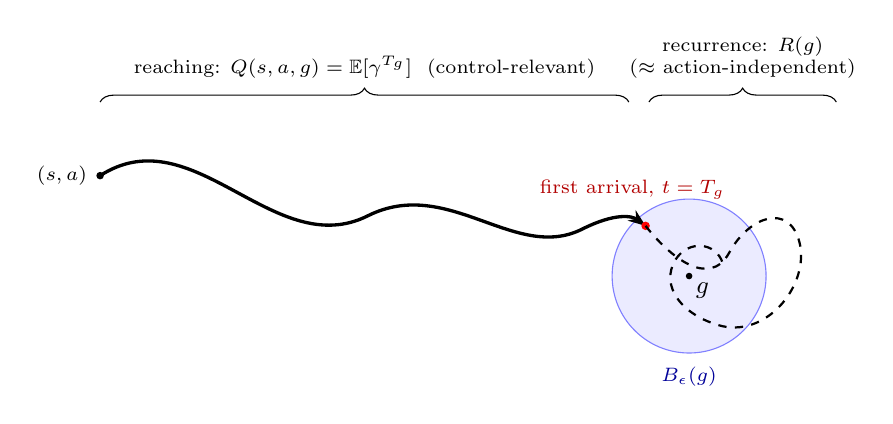
\begin{tikzpicture}[scale=0.85, font=\small]
  % goal ball
  \draw[fill=blue!8, draw=blue!50] (5.2,0) circle (1.15);
  \fill (5.2,0) circle (1.4pt);
  \node[below right, inner sep=1pt] at (5.25,-0.05) {$g$};
  \node[font=\scriptsize, blue!60!black] at (5.2,-1.5) {$B_\epsilon(g)$};
  % start marker
  \fill (-3.6,1.5) circle (1.6pt);
  \node[left, font=\scriptsize] at (-3.65,1.5) {$(s,a)$};
  % approach path (solid): long, indirect
  \draw[very thick, -{Stealth[length=2.2mm]}]
    (-3.6,1.5) .. controls (-2.2,2.4) and (-1.0,0.2) .. (0.4,0.9)
               .. controls (1.6,1.5) and (2.6,0.2)  .. (3.6,0.7)
               .. controls (4.1,0.95) and (4.35,0.9) .. (4.55,0.75);
  \fill[red] (4.55,0.75) circle (1.8pt);
  \node[above, font=\scriptsize, red!70!black] at (4.35,1.0) {first arrival, $t=T_g$};
  % dwell / revisit loops (dashed): in and out of the ball
  \draw[thick, dashed]
    (4.55,0.75) .. controls (4.9,0.3)  and (5.5,-0.2) .. (5.8,0.35)
                .. controls (6.1,0.9)  and (6.7,1.1)  .. (6.85,0.5)
                .. controls (7.0,-0.1) and (6.4,-0.9) .. (5.7,-0.75)
                .. controls (5.1,-0.6) and (4.75,-0.15) .. (5.0,0.25)
                .. controls (5.2,0.55) and (5.6,0.5)  .. (5.7,0.2);
  % braces
  \draw[decorate,decoration={brace,amplitude=5pt}] (-3.6,2.6) -- (4.3,2.6)
     node[midway, above=5pt, font=\scriptsize]
     {reaching: $Q(s,a,g)=\E[\gamma^{T_g}]$ \ (control-relevant)};
  \draw[decorate,decoration={brace,amplitude=5pt}] (4.6,2.6) -- (7.4,2.6)
     node[midway, above=5pt, font=\scriptsize, align=center]
     {recurrence: $R(g)$\\ ($\approx$ action-independent)};
\end{tikzpicture}
\caption{The occupancy of a small goal region splits at the first arrival:
everything before $T_g$ is the \emph{reaching} problem (solid), which is what control must
solve; everything after (dashed: dwelling and revisiting, prominent in play data) contributes
only the goal-dependent recurrence mass $R(g)$.
Eq.~\ref{eq:factor}: $M = Q\cdot R$.
On our data $R$ has mean $\approx 24.7$ discounted visits --- most of the magnitude of $M$
carries no control signal.}
\label{fig:ball}
\end{figure}

Two empirical facts about play data make this decomposition load-bearing:

\begin{enumerate}
  \item \textbf{The recurrence factor is large and nearly action-independent.}
  Play trajectories dwell and revisit: the Monte-Carlo estimate of the second factor on our data has mean $\approx 24.7$ (in units of discounted visits, $\gamma=0.99$) with large variance across goals.
  Fitting a goal-only regressor $R(g)$ explains occupancy well (rank correlation $\approx 0.6$ with Monte-Carlo occupancy, uniformly across horizon buckets), while the reaching term alone explains almost none of it ($\approx 0.06$).
  So most of the \emph{magnitude} of occupancy carries no control signal.

  \item \textbf{The standard estimator spends its capacity on exactly that part.}
  The density-based TD used by FB-style methods handles the on-diagonal (observed successor) term \emph{linearly} --- the loss contains $-\E[M]$, a term that always pays for making $M$ larger --- and is stabilized only by an orthonormality regularizer on the state embedding.
  On this domain that regularizer is itself destructive (below).
  Removing it un-anchors the linear term: we verified that even with a \emph{frozen, known-good} goal embedding, the density-based TD inflates without bound (critic scale $154\to 5\times10^{4}$ within 65k steps) and control degrades monotonically ($0.98\to0.42$ by 100k steps).
\end{enumerate}

The design that falls out: \emph{learn the reaching term first, with a bounded regression objective; then learn occupancy on top of it, using an objective in which every term is a squared residual against a representable $0/1$ reward.}

\section{From density-ratio TD to finite-region regression}
\label{sec:density-to-kernel}

Section~\ref{sec:intuition} argued \emph{empirically} that the density estimator
spends its capacity on recurrence and inflates without an external anchor.
This section derives \emph{why} from the successor-measure Bellman equation, and shows
that a single substitution --- a finite goal region in place of a point query --- turns
every entry of the training matrix into a bounded squared residual, which is what phases
1 and 2 exploit.
It also states the objects in the separated $F^{\top}B$ form, connecting the diagonal
slice trained below (Section~\ref{sec:algo}) to the full FB object
(Section~\ref{sec:dense}).

\paragraph{The singular immediate term.}
Write $m_z(s,a,x)=dM^{\pi_z}(s,a,\cdot)/d\rho\,(x)$ for the density of the successor
measure relative to a reference $\rho$; this is the object FB factorizes as
$F(s,a,z)^{\top}B(x)$.
It satisfies the density Bellman equation
\[
m_z(s,a,x)
\;=\;
\frac{\delta_{s'}(x)}{\rho(x)}
\;+\;
\gamma\,\E_{a'\sim\pi_z(\cdot\mid s')}\big[m_z(s',a',x)\big].
\]
The immediate term is a \emph{Dirac density ratio}: on the observed successor it is a
point mass divided by $\rho$, not a finite scalar that can be placed inside a squared
Bellman residual.
FB therefore does not regress this equation directly.
It minimizes the least-squares density-matching surrogate
\[
\tfrac12\,\E_{x\sim\rho}\big[(m_z-\gamma m_z')^2\big]
\;-\;
\E\big[m_z(s,a,s')-\gamma m_z'(s,a,s')\big]
\;+\;
\lambda_{\mathrm{ortho}}\,\mathcal{L}_{\mathrm{ortho}},
\]
in which the off-diagonal (random-query) entries carry the quadratic residual and the
observed successor enters only through the \emph{negative linear} term --- the same
$-\E[M]$ flagged in Section~\ref{sec:intuition}.
This term has no fixed target; it pays unconditionally for making the matched-successor
value larger, and its scale is held in check \emph{only} by the orthonormality
regularizer on $B$.
Remove that regularizer and nothing bounds the diagonal --- precisely the divergence we
observe on a frozen, known-good embedding (critic scale $154\to5\times10^{4}$;
Section~\ref{sec:exp-mech}).
The two standard stabilizers are thus load-bearing in opposite directions: ortho anchors
the scale but destroys the reaching geometry (the $2\times2$ of Section~\ref{sec:exp-p1}).

\paragraph{The substitution.}
Replace the point query by a finite region.
With the cube-position ball $B_\epsilon(g)$ and the hit indicator
$h(s',g)=\ind{\|\mathrm{cube}(s')-\mathrm{cube}(g)\|\le\epsilon}\in\{0,1\}$ of
Section~\ref{sec:algo}, the singular immediate term $\delta_{s'}(x)/\rho(x)$ becomes the
bounded scalar $h(s',g)$.
Every entry of the matrix --- diagonal included --- now has an explicit target and is an
ordinary squared residual: no separate linear diagonal term, no off-diagonal mask, and the
$0/1$ event pins the scale directly, so no orthonormality (or any) regularizer on $B$ is
needed.
This substitution is the whole content of the change,
\[
\text{density-ratio estimation}
\;\longrightarrow\;
\text{Bellman regression on finite goal regions}.
\]
The two phases are then the same regression under two backups, differing only in whether
arrival absorbs:
\[
y^{\mathrm{reach}}_{ij}=h_{ij}+\gamma(1-h_{ij})\,\bar Q_{ij},
\qquad
y^{\mathrm{visit}}_{ij}=h_{ij}+\gamma\,\bar M_{ij}.
\]
Phase 1 (Algorithm~1) terminates the backup at first arrival, giving the bounded reaching
value $Q=\E[\gamma^{T_g-1}]\in[0,1]$; phase 2 (Algorithm~2) drops the $(1-h_{ij})$ factor
so revisits keep accumulating, giving the visitation value $M\in[0,1/(1-\gamma)]$.
The kernel event is what makes both objects bounded and self-anchored --- the property the
density form structurally lacks.

\paragraph{Same architecture, separated arguments.}
Nothing above ties the policy index to the query.
In full FB form the two objects are $Q(s,a,z,x)$ and
$M(s,a,z,x)=F(s,a,z)^{\top}B(x)/\sqrt d$ with $z$ and $x$ \emph{independent};
the diagonal slice $z=\psi(g),\,x=g$ trained in
Sections~\ref{sec:algo}--\ref{sec:exp-p2} is the special case in which the policy and the
query name the same goal.
The reach-first substitution therefore applies verbatim to the separated form of
Section~\ref{sec:dense} --- only the batch's row-index ($z_j$) and column-query ($x_k$)
sampling changes, not the loss.

\section{The structure in a 50-state playpen}
\label{sec:playpen}

Before the algorithm, the structural claims of Sections~\ref{sec:intuition} and
\ref{sec:density-to-kernel} can be exhibited \emph{exactly} in a minimal MDP built to
have the same anatomy as manipulation play data
(\texttt{scripts/rescuing\_fb/tabular\_playpen.py}; everything below is a linear solve
unless marked SGD).

\textbf{The playpen MDP.} A $7\times7$ grid plus a pit ($50$ states, $5$ actions:
stay/up/down/left/right). The \emph{semantic coordinate} is the \textbf{column} (the
cube-position analog: goal regions are columns); the \emph{interaction mode} is the
\textbf{row} (the grasp/velocity analog, invisible to the region). A $2\times2$
\textbf{bowl} is sticky --- move attempts leave with probability $0.1$ (a cube at
rest); the top row is a \textbf{conveyor} that drifts two columns per step regardless
of the action (a carried cube: fast transport, but position cannot be held), and
riding off its end drops into a hard-to-leave pit (a dropped cube must be re-fetched).
The ``play'' behavior policy is a goal-directed mixture of reach-a-column policies
plus exploration noise; $\gamma=0.99$.

\textbf{(i) The factorization is exact, and recurrence carries the magnitude.}
For singleton goals the renewal identity $M=Q\cdot R$ of Eq.~\ref{eq:factor} holds to
numerical precision (max error $1.4\times10^{-9}$). Recurrence spans a wide range
($R\approx16.5$ in the bowl vs.\ $1.9$ on the conveyor) while reaching values compress
toward $1$ at this horizon. Across the seven column regions under the play policy, a
\emph{goal-only} recurrence predictor ranks occupancy at Spearman $\mathbf{0.96}$
while the reaching term alone ranks it at $0.58$ ($R$ spans $4.2$--$30.7$; reaching
spans $0.34$--$1$) --- the playpen version of the $0.60$-vs-$0.06$ statistic of
Section~\ref{sec:exp-mech}, here exact rather than estimated.

\textbf{(ii) Arrival ranking and occupancy ranking genuinely disagree.}
Weight two regions --- the bowl (stable) and one conveyor cell (transient) --- by
$w_{\mathrm{bowl}}{=}1$, $w_{\mathrm{conv}}{=}2.11$, chosen between the reaching ratio
($1.04$: the conveyor cell is nearly as \emph{reachable}) and the occupancy ratio
($4.26$). Ranking candidates by weighted reaching value picks the conveyor; ranking by
weighted occupancy picks the bowl; exact policy evaluation confirms the bowl
($96.8$ vs.\ $47.9$ discounted return). A goal-reaching value, however well trained,
selects the wrong region here by construction --- this is the tier-3 task of the
evaluation suite (spec 11) in miniature. The diagonal-slice defect of
Section~\ref{sec:object} is also exact: summing the two slices values the pair at
$144.7$, while no single policy can achieve more than $96.8$.

\textbf{(iii) The bounded regression dominates the density surrogate at matched rank
(SGD).} Fitting rank-$8$ bilinear $F^{\top}B$ on $20$k offline play transitions
(fixed policy, $\gamma=0.95$, Adam, identical architecture and data): the
column-region visitation regression reaches relative error $0.05$--$0.09$ and
per-state goal-ranking correlation $0.96$--$0.99$; the FB density-TD reaches only
$0.38$ / $0.65$, and \emph{adding} the orthonormality regularizer makes it worse
($0.53$ / $0.45$) --- ortho damaging the geometry exactly as in the $2\times2$ of
Section~\ref{sec:exp-p1}. Two honest notes: with no actor in the loop the density
estimator here \emph{fits poorly but does not diverge} (its output scale settles
$\sim8\times$ the region form's, with a target dynamic range of $\sim80$ vs.\ a
bounded target of $\le12$), consistent with the divergence of
Section~\ref{sec:exp-mech} being a property of the estimator-plus-actor system; and
absorbing-first curriculum and direct visitation regression perform alike in this
pure-evaluation setting ($0.09$ vs.\ $0.05$), consistent with the curriculum's value
lying in the control loop, not in policy evaluation.

\section{Algorithm}
\label{sec:algo}

Figure~\ref{fig:pipeline} shows the full pipeline; the two phases are specified in
Algorithms~1 and~2.

\begin{figure}[t]
\centering
\resizebox{\textwidth}{!}{%
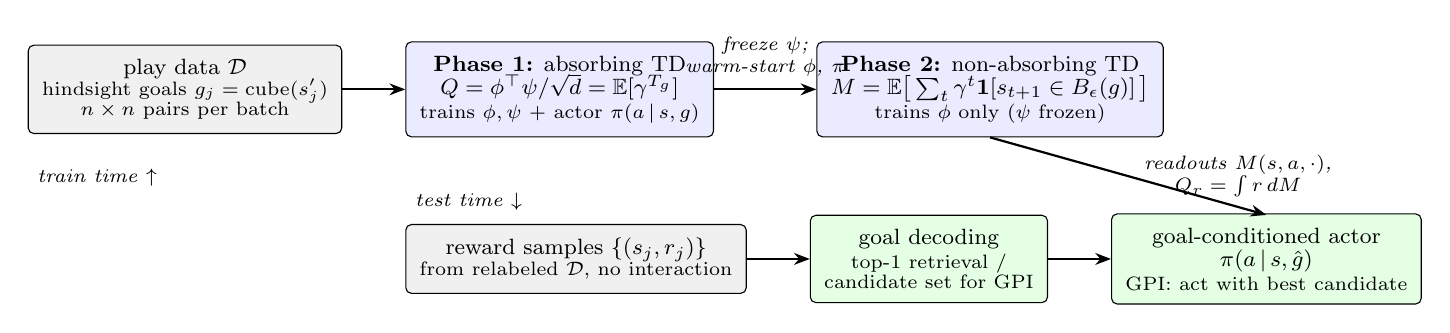
\begin{tikzpicture}[
  font=\footnotesize,
  box/.style={draw, rounded corners=2pt, align=center, inner sep=5pt},
  data/.style={box, fill=gray!12},
  ph/.style={box, fill=blue!8},
  ex/.style={box, fill=green!10},
  arr/.style={-{Stealth[length=2mm]}, thick},
  lab/.style={font=\scriptsize\itshape, align=center}
]
  % training row
  \node[data] (data) {play data $\mathcal{D}$\\[-2pt]{\scriptsize hindsight goals $g_j=\mathrm{cube}(s_j')$}\\[-2pt]{\scriptsize $n\times n$ pairs per batch}};
  \node[ph, right=8mm of data] (p1) {\textbf{Phase 1:} absorbing TD\\[-1pt]
    $Q=\phi^{\top}\psi/\sqrt{d}=\E[\gamma^{T_g}]$\\[-1pt]
    {\scriptsize trains $\phi,\psi$ + actor $\pi(a\,|\,s,g)$}};
  \node[ph, right=13mm of p1] (p2) {\textbf{Phase 2:} non-absorbing TD\\[-1pt]
    $M=\E\big[\sum_t \gamma^{t}\ind{s_{t+1}\in B_\epsilon(g)}\big]$\\[-1pt]
    {\scriptsize trains $\phi$ only ($\psi$ frozen)}};
  \draw[arr] (data) -- (p1);
  \draw[arr] (p1) -- node[lab, above=1pt] {freeze $\psi$;\\ warm-start $\phi$, $\pi$} (p2);
  % test-time row
  \node[data, below=11mm of p1.south west, anchor=north west]
    (rew) {reward samples $\{(s_j, r_j)\}$\\[-2pt]{\scriptsize from relabeled $\mathcal{D}$, no interaction}};
  \node[ex, right=8mm of rew] (dec) {goal decoding\\[-1pt]{\scriptsize top-$1$ retrieval /}\\[-2pt]{\scriptsize candidate set for GPI}};
  \node[ex, right=8mm of dec] (pol) {goal-conditioned actor\\[-1pt]$\pi(a\,|\,s,\hat g)$\\[-1pt]{\scriptsize GPI: act with best candidate}};
  \draw[arr] (rew) -- (dec);
  \draw[arr] (dec) -- (pol);
  \draw[arr] (p2.south) -- node[lab, right=2pt] {readouts $M(s,a,\cdot)$,\\ $Q_r=\int r\,dM$} ($(pol.north)+(0,-0.02)$);
  % phase separator
  \node[lab, anchor=west] at ($(data.south west)+(0,-0.55)$) {train time $\uparrow$};
  \node[lab, anchor=west] at ($(rew.north west)+(0,0.28)$) {test time $\downarrow$};
\end{tikzpicture}}
\caption{Pipeline. Training (top): phase 1 learns the goal-reaching value and the policy;
phase 2 re-trains the forward tower $\phi$ into a visitation measure on the frozen goal
embedding $\psi$.
Test time (bottom): a reward specified by labeled dataset samples is reduced to one or a few
candidate goals (retrieval / GPI), executed by the goal-conditioned actor; the measure
readouts score candidates and integrate rewards.}
\label{fig:pipeline}
\end{figure}
Both phases use the bilinear critic
\[
Q_\theta(s,a,g)=\phi(s,a)^{\top}\psi(g)/\sqrt{d}
\]
(two-layer MLP, $d=50$, twin heads with $\min$-backup), and both are trained on minibatch ``matrices'': for a batch of $n$ transitions $(s_i,a_i,s_i')$, the columns are the $n$ relabeled goals $g_j=\mathrm{cube}(s_j')$ (hindsight relabeling \citep{andrychowicz2017hindsight}), giving $n\times n$ residuals per batch --- the diagonal pairs each transition with its own future, the off-diagonal supplies random goals.
The policy is a flow-matching behavior-cloning policy with one-step distillation and a greedy term on the critic readout, following flow Q-learning \citep{park2025flow}; the greedy term is normalized by the (stop-gradient) magnitude of $Q$ to be scale invariant.

\begin{algorithm}[h]
\caption{Phase 1 --- goal-reaching value (absorbing formulation)}
\begin{algorithmic}[1]
\For{each gradient step}
  \State sample batch $\{(s_i,a_i,s_i')\}_{i=1}^{n}$; goals $g_j=\mathrm{cube}(s_j')$; $h_{ij}=\ind{\,\|\mathrm{cube}(s_i')-g_j\|\le\epsilon\,}$
  \State $a_i' \sim \pi(\cdot \mid s_i', g)$ \Comment{bootstrap action from the current policy}
  \State $y_{ij} = h_{ij} + \gamma\,(1-h_{ij})\,\bar Q(s_i',a_i',g_j)$ \Comment{absorbing: reaching the ball ends the backup}
  \State $\mathcal{L}_Q=\frac{1}{n^2}\sum_{ij}\big(Q(s_i,a_i,g_j)-\sg[y_{ij}]\big)^{2}\,/\,\sg[\overline{Q^{2}}]$
  \State update $\phi,\psi$ on $\mathcal{L}_Q$; update policy (flow BC + distilled greedy step on $Q$)
\EndFor
\end{algorithmic}
\end{algorithm}

The fixed point is $Q(s,a,g)=\E[\gamma^{T_g-1}]\in[0,1]$ (the immediate-hit case $T_g{=}1$
receives target $1$, so the discount counts from the current transition; this is the
convention under which the affine identity of Section~\ref{sec:baseline},
$Q=1+(1-\gamma)V$, is exact).
The sparse $0/1$ arrival reward is representable, so \emph{every} entry --- diagonal
included --- is a plain squared residual; the idealized backup operator is a
$\gamma$-contraction; the reward pins the scale, so no orthonormality (or any other)
regularizer on $\psi$ is used.

\begin{algorithm}[h]
\caption{Phase 2 --- visitation measure on the frozen goal embedding}
\begin{algorithmic}[1]
\State initialize all networks from phase 1; \textbf{freeze} $\psi$
\For{each gradient step}
  \State sample batch, goals, $h_{ij}$ as in phase 1
  \State $y_{ij} = h_{ij} + \gamma\,\bar M(s_i',a_i',g_j)$ \Comment{\emph{non}-absorbing: revisits keep counting}
  \State $\mathcal{L}_M=\frac{1}{n^2}\sum_{ij}\big(M(s_i,a_i,g_j)-\sg[y_{ij}]\big)^{2}\,/\,\sg[\overline{M^{2}}]$
  \State update $\phi$ (and the policy; greedy term normalized by the \emph{centered} magnitude $\sg\,\E|M-\bar M|$)
\EndFor
\end{algorithmic}
\end{algorithm}

The phase-2 fixed point is the discounted visitation count
\[
M(s,a,g)=\E\left[\sum_{t\ge0}\gamma^{t}\ind{s_{t+1}\in B_\epsilon(g)}\right]
\]
--- a visitation value (occupancy of the ball, revisits counted), bounded by
$1/(1-\gamma)$, with squared residuals only.
The contraction statement applies to the idealized fixed-policy evaluation operator; the
practical estimator (changing actor, rank-$50$ bilinear approximation, twin-min backups,
offline bootstrap actions, a $\psi$ trained for a different target) carries no such
guarantee --- stability is an empirical finding here, not a theorem.
Freezing $\psi$ carries the phase-1 goal geometry into phase 2 and isolates what changed if phase 2 misbehaves.
The centered actor normalization compensates for the fact that, per Eq.~\ref{eq:factor}, $M$ carries a large shared recurrence baseline that would otherwise dilute the greedy signal.
(A variant we have not yet run keeps the phase-1 \emph{actor} frozen too and trains only a
separate visitation head: if the recurrence factor really is action-independent, phase-2
actor updates can only add drift, and this variant would isolate that.)

An alternative phase 2, which requires no TD at all: keep $Q$ from phase 1 and fit the scalar recurrence factor $R(g)$ of Eq.~\ref{eq:factor} by Monte-Carlo regression on the frozen $\psi(g)$, using $M\approx Q\cdot R$.
This is cheaper but only approximate; the TD version is exact in the limit and is our primary variant.

\section{Experiments}
\label{sec:experiments}

\subsection{Setup, protocol, and nomenclature}

\textbf{Environment and data.} All experiments use OGBench
\texttt{cube-single-play-v0}: a 6-DoF arm and one cube, 28-dimensional state
observations, and an offline dataset of $10^{6}$ transitions collected by a scripted
``play'' policy that repeatedly picks the cube up, moves it, and sets it down
(Figure~\ref{fig:ball} and the report strips show what this looks like).
No reward labels are used at training time.

\textbf{Training.} Unless stated otherwise: bilinear critic
$\phi(s,a)^{\top}\psi(g)/\sqrt d$ with $d{=}50$, twin heads with $\min$-backup,
$\gamma=0.99$, goal ball $\epsilon=4$\,cm on the cube position, hindsight-relabeled
batch goals ($n\times n$ residuals per batch), flow-BC + one-step-distillation actor,
500k gradient steps, 2--3 seeds per cell.
Curves are evaluated every 50k steps.

\textbf{Evaluation.} Five harnesses are used in this note, measuring different
things; Table~\ref{tab:harnesses} is the index, and the two that carry the
headline numbers are described immediately below.

\begin{table}[h]
\centering\footnotesize
\setlength{\tabcolsep}{4pt}
\renewcommand{\arraystretch}{1.2}
\begin{tabular}{l p{3.5cm} p{3.4cm} l}
\toprule
\textbf{Harness} & \textbf{What it scores} & \textbf{Protocol} & \textbf{Where} \\
\midrule
Native GC & the \emph{actor}, on the 5 built-in tasks & 50 episodes/task, mean success & everywhere \\
Zero-shot (goal-decode) & inference {+} decode over 6 goal-reducible families & $m{=}2000$ labels, 25 ep., $H{=}200$ & \S\ref{sec:exp-zs}, Tab.~\ref{tab:rewards} \\
Set-mass calibration (L1) & whether $\tilde M$ \emph{is a measure} & 32 starts $\times$ 3 rollouts vs.\ MC, 3 box scales & \S\ref{sec:exp-calib} \\
Novel-reward transfer (L2) & the \emph{readout}, on 48 unseen rewards & prediction {+} control, 3 baselines & \S\ref{sec:exp-l2}, Tab.~\ref{tab:l2} \\
Measure benchmark (SMB) & measure quality across variants & Wing-B: B1--B3 & \S\ref{sec:smb} \\
\bottomrule
\end{tabular}
\caption{The evaluation suite. The first two score behavior, the last three score
the object. They are not interchangeable, and \S\ref{sec:exp-calib} shows they
can disagree.}
\label{tab:harnesses}
\end{table}

(i) \emph{Native goal-conditioned evaluation}: the five OGBench \texttt{cube-single}
tasks, 50 episodes per task, overall success = mean task success; this is the number
reported for every training curve and final checkpoint.
(ii) \emph{Zero-shot harness}: a task is specified only by reward labels on $m{=}2000$
states relabeled from the offline dataset; the harness infers a task representation,
extracts a policy without any training, and rolls out 25 episodes per task variant at
horizon 200 in batched lock-step environments.
The six reward families are defined in Table~\ref{tab:rewards} and visualized on the
cube workspace in Figure~\ref{fig:rewards}; $c(x)$ denotes the cube position of state
$x$, $c^{*}$ a task-goal cube position, and $\epsilon=4$\,cm throughout.

\begin{table}[h]
\centering
\footnotesize
\setlength{\tabcolsep}{4pt}
\renewcommand{\arraystretch}{1.35}
\begin{tabular}{l l p{3.3cm} p{4.5cm}}
\toprule
\textbf{Family} & \textbf{Reward $r(x)$} & \textbf{Success criterion} & \textbf{What we see} \\
\midrule
\textsc{dirac} & $\ind{\|c(x)-c^{*}\|\leq\epsilon}$ &
  environment success flag at $c^{*}$ (identical to the native eval) &
  solved: $0.89$--$0.97$ retrieval, $0.90/0.92$ direct-$z$ \\
\textsc{mixture} & $\max_{k\in\{1,2\}}\ind{\|c(x)-c_k\|\leq\epsilon}$ &
  success at \emph{either} goal (all 10 task pairs) &
  $0.64$--$0.89$ family mean; easiest pairs $0.94$--$1.00$ \\
\textsc{region} & $\ind{c(x)\in R}$, $R$ = 6\,cm box or 4\,cm ball &
  cube inside $R$ at episode end &
  $0.73$--$0.80$ retrieval --- below every goal-reducible family \\
\textsc{dense} & $\exp\!\big(-\|c(x)-c^{*}\|/\sigma\big)$, $\sigma{=}8$\,cm &
  environment success flag at the peak $c^{*}$ &
  $0.93$--$0.99$ retrieval; direct-$z$ seed-split $0.90/0.13$ \\
\textsc{linear} & $\psi(x)^{\top}\tilde z/\sqrt{d}$, random unit $\tilde z$ &
  no success flag exists; achieved discounted reward vs.\ a random-$z$ control &
  unresolved: beats control on 2/3 phase-1 seeds, enormous variance, no edge on the
  separated form \\
\textsc{reach-avoid} & $\ind{c(x)\in A}-\ind{c(x)\in B}$ &
  success-at-$A$; fraction of episode time in $B$ (exploratory) &
  reach side $0.91$--$0.96$ retrieval; avoid side non-discriminative (time-in-$B$
  $\leq 0.003$ for \emph{every} policy) \\
\bottomrule
\end{tabular}
\caption{The zero-shot reward families: definition, scoring, and the one-line
observation. Per-route, per-seed numbers in Table~\ref{tab:zs}.}
\label{tab:rewards}
\end{table}

\begin{figure}[t]
\centering
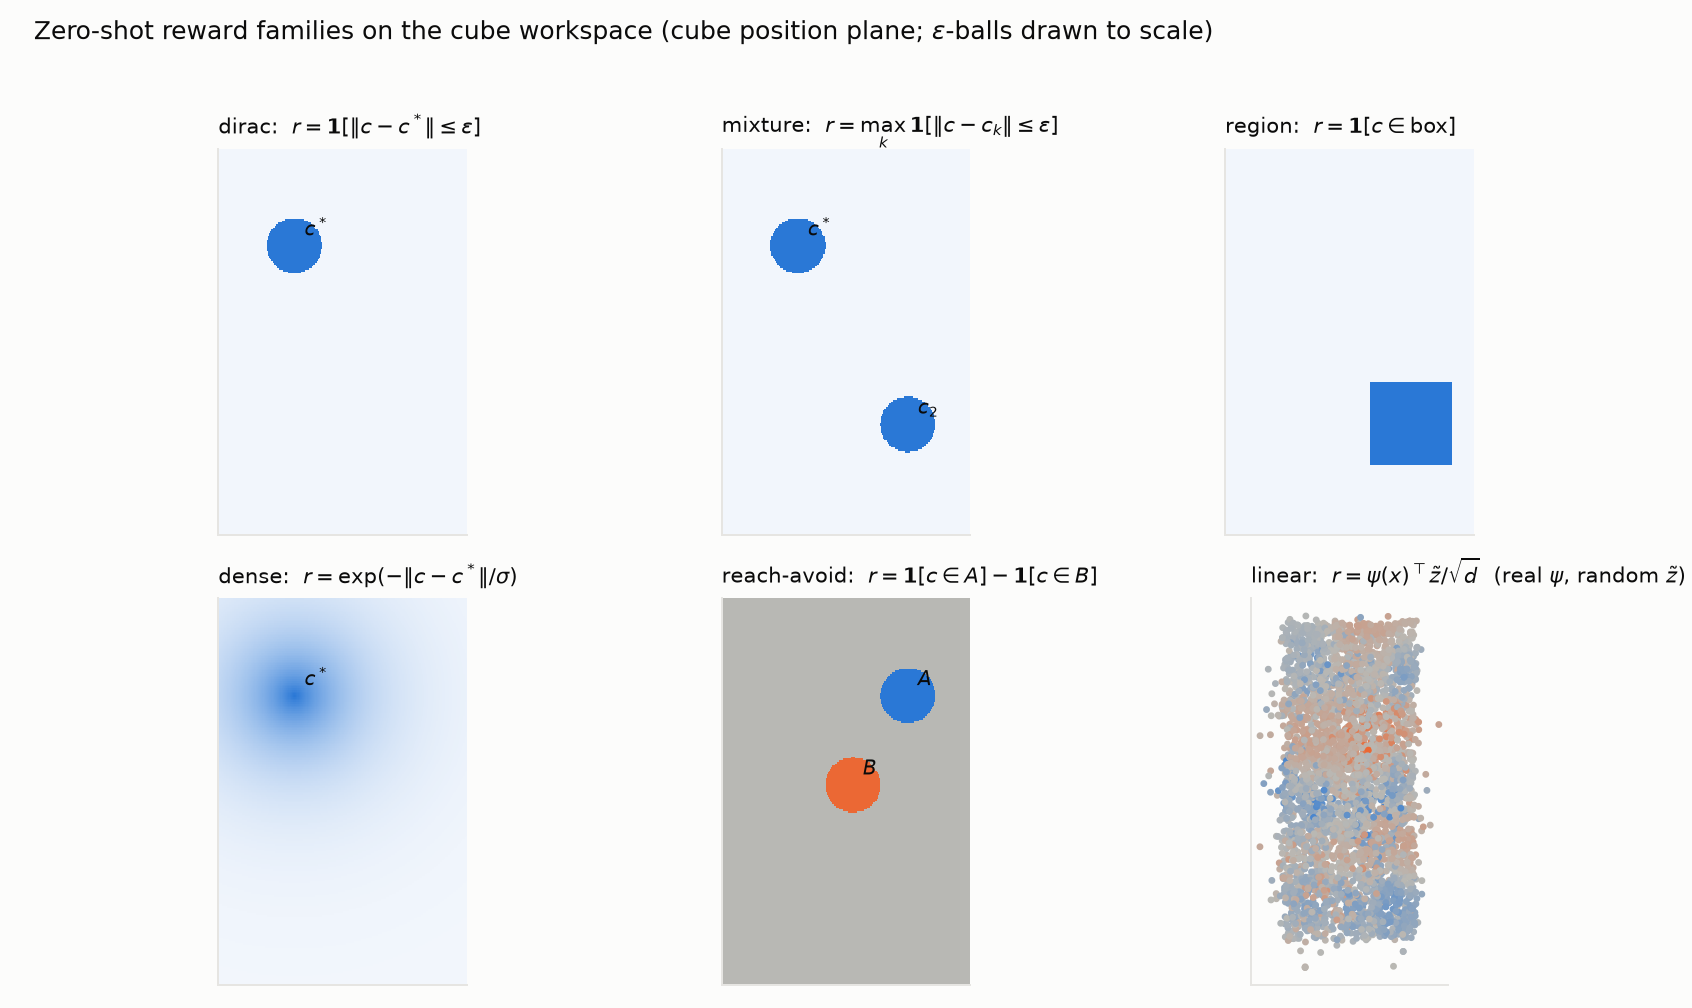
\includegraphics[width=0.95\textwidth]{figures/5_rewards.png}
\caption{What each reward family looks like on the cube workspace (cube-position
plane; $\epsilon$-balls to scale). The first five are functions of cube position.
The \textsc{linear} panel is computed with the \emph{trained} phase-1 embedding:
dataset states colored by $\psi(x)^{\top}\tilde z$ for one random direction
$\tilde z$ --- the field is spatially incoherent in cube space, which is the visual
form of the extraction boundary: no reduction of this reward to a goal (or any small
candidate set) exists, so only genuine measure integration can serve it.}
\label{fig:rewards}
\end{figure}
Inference variants: \emph{moment/regression} $z_r$ in embedding space (consumed
directly or decoded); \emph{retrieval-$k$} (mean embedding of the top-$k$
reward-weighted dataset states; $k{=}1$ decodes to the single best state as a goal);
\emph{GPI} over a candidate set (act with the candidate whose critic readout is
highest in the current state).

All numbers below are overall success on this protocol unless noted.

\subsection{Anchors}
\label{sec:exp-anchors}

Goal-conditioned IQL with the same bilinear critic and the same actor class reaches
$\mathbf{0.904}$; the FB representation trained on the same data with the same actor
class plateaus at $\approx 0.42$.
These two numbers frame everything below: the gap is the phenomenon, and $0.90$ is the
bar a measure-trained critic must meet.

\subsection{The measure-objective ladder (the negative record)}
\label{sec:exp-ladder}

Before proposing anything, we ran the canonical repairs, each as a single-axis move on
the same measure-only cell (bilinear $d{=}50$, state-action measure on the critic legs,
3 seeds each unless noted).
Table~\ref{tab:ladder} is the complete record.

\begin{table}[h]
\centering
\small
\setlength{\tabcolsep}{6pt}
\renewcommand{\arraystretch}{1.12}
\begin{tabular}{l c l}
\toprule
\textbf{Variant} & \textbf{Success} & \textbf{Note} \\
\midrule
density-TD occupancy (FB form, with orthonormality) & $\le 0.10$ & the starting point \\
\quad + conservatism ($\min$-aggregation) & $0.240$ & pessimism \emph{hurts} \\
\quad faithful one-step variant & $0.067$ & $\approx$ BC floor \\
\quad hindsight test-point columns alone & $0.095$ & \\
\quad in-sample expectile backup alone & $0.103$ & \\
\quad paired$\leftrightarrow$random column dial, deconfounded\textsuperscript{a} & $0.00$ & every setting flat \\
\quad reaching semantics alone (regularizer still on) & $0.225$ & the first cell off the floor \\
task-embedding grounding mixed into the critic & collapses & $0.96$ mid-run $\to 0.0$--$0.4$ (7/7 seeds) \\
embedding-conditioned actor under a sampling prior & $0.395$ & the prior, not the conditioning (\S\ref{sec:exp-sep}) \\
\bottomrule
\end{tabular}

\vspace{2pt}
\raggedright\footnotesize
\textsuperscript{a} rerun with the regularizer off and the loss-scale defect fixed, so
the earlier confound is removed; includes the full-corner combination (reaching +
expectile + hindsight columns), which also sits at $0.00$ --- stacking axes on the
reaching cell \emph{destroys} it.
\label{tab:ladder}
\end{table}

The single informative rung: changing the \emph{semantics} of the target from
occupancy to first arrival ($0.225$, sustained, despite a $\sim$100$\times$ oversized
regularizer in the changed units).
That rung became phase 1.

\subsection{Phase 1: the reaching value --- the deciding $2\times2$}
\label{sec:exp-p1}

The two candidate explanations for $0.225$ vs.\ the $0.90$ bar were the target
semantics and the orthonormality regularizer.
The $2\times2$ (3 seeds per cell, 500k):

\begin{center}
\small
\begin{tabular}{l c c}
\toprule
 & no regularizer & with regularizer \\
\midrule
reaching semantics & $\mathbf{0.967 \pm 0.012}$ \ (0.956/0.964/0.980) & $0.225$ \\
occupancy semantics & floored / unstable & $\approx 0.10$ \\
\bottomrule
\end{tabular}
\end{center}

Both ingredients are necessary; neither suffices.
The winning cell crosses $0.94$ by 50k steps and is stable to 500k
(Figure~\ref{fig:curves}).
\textbf{Verification.} Because a single surprising cell can be an evaluation artifact,
each of the three checkpoints was re-evaluated in a separate process with fresh
environment seeds (100 episodes/task for seed 0, 50 for seeds 1--2):
$0.972 / 0.988 / 0.984$.
Six additional incidental step-0 re-evaluations during later warm-starts read
$0.96$--$0.99$.

\begin{figure}[t]
\centering
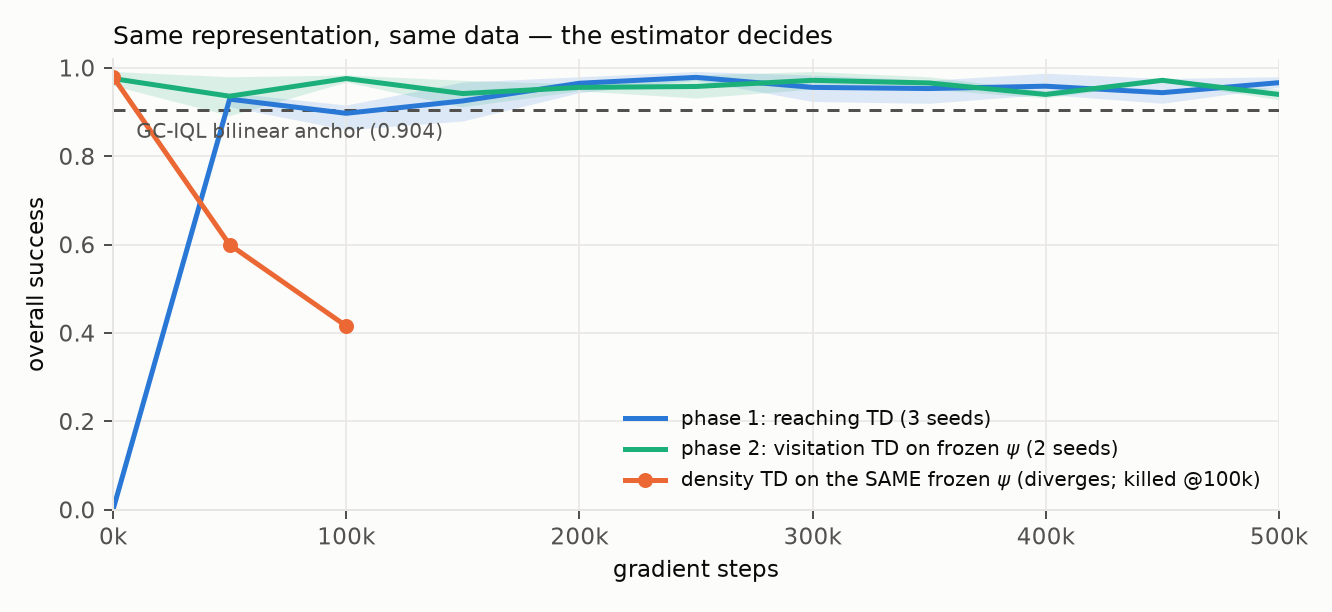
\includegraphics[width=0.85\textwidth]{figures/2_curves.png}
\caption{Native-evaluation success against gradient steps.
One representation, one dataset, three training signals: the reaching TD (blue, 3
seeds) and the visitation TD on the frozen reaching geometry (aqua, 2 seeds) sit at
the GC-IQL anchor for the full run; the density-form TD on the \emph{same frozen
geometry} (orange) degrades immediately and monotonically.}
\label{fig:curves}
\end{figure}

\subsection{Mechanism evaluations}
\label{sec:exp-mech}

\textbf{The frozen-$\psi$ divergence experiment.}
Warm-start every network from a finished phase-1 checkpoint, freeze $\psi$, and train
$\phi$ with the density-form TD (the FB estimator: linear observed-successor term,
squared off-diagonal term, no regularizer).
If the historical failures were representational, this cell must succeed --- the
representation is, by construction, one that supports $0.97$ control.
Instead the critic scale inflates $154\to5.4\times10^{4}$ within 65k steps and success
decays $0.98\to0.60\to0.42$ by 100k (3 seeds; Figure~\ref{fig:scale}).
A control with $\psi$ \emph{trainable} collapses faster still ($0.97\to0.07$ and
$0.98\to0.06$ at 50k, 2 seeds): representation corruption compounds the estimator
defect but is not its cause.

\begin{figure}[t]
\centering
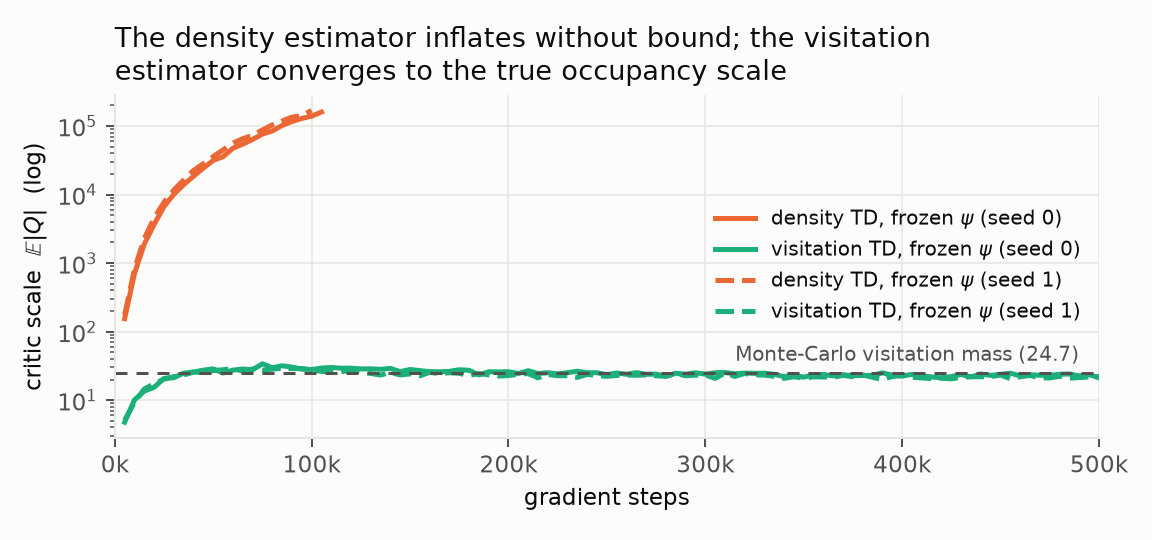
\includegraphics[width=0.8\textwidth]{figures/4_scale.png}
\caption{Critic scale $\E|Q|$ (log) during phase-2-style training on the frozen
phase-1 embedding. The density estimator (orange) inflates without bound --- its
linear term pays unconditionally for larger $M$ once the orthonormality anchor is
removed. The visitation estimator (aqua) plateaus on the Monte-Carlo estimate of the
true discounted visitation mass (dashed): it converges to the correct measure, not a
rescaled surrogate.}
\label{fig:scale}
\end{figure}

\textbf{Revisit-mass statistics.}
Monte-Carlo, over the dataset at the $4$\,cm goal ball: discounted occupancy
accumulated \emph{after} first arrival has mean $\approx 24.7$ (within-trajectory
estimate $\approx 30$, bimodal: ``passed through'' vs.\ ``settled''), with large
variance across goals.
A goal-only regressor $R(g)$ of this mass, fit on the frozen $\psi(g)$, predicts
Monte-Carlo occupancy at Spearman rank correlation $0.60$--$0.63$ \emph{uniformly
across horizon buckets} (including first-arrival times $>20$ steps), while the
reaching term alone predicts at $0.06$; a position-only regressor fits $13\times$
worse (MSE $0.93$ vs.\ $0.069$) than the $\psi$-input one.
This is the quantitative content of Eq.~\ref{eq:factor}: the recurrence factor
carries essentially all of occupancy's magnitude, and the learned embedding supports
predicting it.

\subsection{Replication in the FB codebase, and what the goal region is doing}
\label{sec:exp-replication}

Every result above was produced in one implementation. We re-implemented the
phase-1/phase-2 objective a second time, inside the FB reference codebase
(PyTorch) rather than the goal-conditioned one (JAX), inheriting FB's own flow
actor, latent sampling, target networks and soft updates unchanged; the sole
edit is the successor residual. This also switches the evaluation protocol: the
numbers in this subsection are FB's \emph{zero-shot} harness, where $z$ is
inferred from $10^4$ reward-relabelled offline transitions, not the native
goal-conditioned eval used elsewhere in this note. Cross-framework numbers are
therefore \textbf{not} interchangeable with the $0.967$ of
Section~\ref{sec:exp-p1}; within this subsection all rows share one protocol and
one anchor, and only those comparisons are made.

Re-implementation also lets us close an ablation this note previously lacked.
The working cell differs from stock FB along \emph{two} axes at once, and the
caveat in Section~\ref{sec:caveats} concedes the two were never separated:

\begin{itemize}\itemsep2pt
\item[(A)] \textbf{reward support.} FB places a Dirac on the exact next state
--- the identity diagonal of the $[B\!\times\!B]$ goal matrix. We replace it
with the $\epsilon$-ball $h(s',g)=\ind{\lVert c(s')-c(g)\rVert\le\epsilon}$,
whose radius ($4$\,cm) matches the evaluation reward's own threshold.
\item[(B)] \textbf{loss form.} FB's quadratic-offdiagonal $+$ \emph{linear}-diagonal
split, with orthonormality and an unbounded fixed point, becomes an
every-entry-squared bounded residual with no regularizer.
\end{itemize}

Only (B) is a novel claim, so (A) needs its own control: \emph{FB's exact loss,
with the Dirac support generalized from $I$ to the ball, everything else stock}
--- linear diagonal, orthonormality on, fixed point unbounded. With $h=I$ this
control reduces algebraically to the stock FB loss (the off-diagonal mask
becomes $1-I$ and the linear term $-\sum_{ij}(\text{diff}\odot I)/\!\sum I$
recovers FB's $-\overline{\mathrm{diag}}\cdot n_{\text{par}}$), so it is a
strict one-axis generalization rather than a re-implementation; that identity is
asserted as a unit test.

\begin{center}
\small
\begin{tabular}{l l l c l}
\toprule
arm & support & loss & mean success & per seed \\
\midrule
stock FB (anchor, 10 seeds) & $I$ & FB & $0.420 \pm 0.055$ & --- \\
\textbf{control} (3 seeds)  & ball & FB & $0.284$ & 0.367 / 0.313 / 0.173 \\
phase 1 (2 seeds)           & ball & bounded, no reg. & $\mathbf{0.922}$ & 0.940 / 0.903 \\
phase 2 (2 seeds)           & ball & visitation, $\psi$ frozen & $0.887$ & 0.867 / 0.907 \\
\bottomrule
\end{tabular}
\end{center}

Mean over evaluations from 250k--500k steps, \texttt{cube-single-play-v0}.
\textbf{The privileged goal region does not explain the gain --- given to FB's
own estimator it makes things worse}, $0.284$ against the $0.420$ anchor. The
bounded residual is what makes a ball-shaped reward usable at all.

The mechanism is visible in the critic scale, and the arms are provably matched
(shared seeds give identical initial values, $3.70$ and $8.63$):

\begin{center}\small
\begin{tabular}{l l}
\toprule
arm & $\overline{|M|}$, start $\to$ 500k \\
\midrule
control (FB loss, ball) & $3.70\to812$, \; $8.63\to1147$, \; $6.80\to1097$ \\
phase 1 (bounded, ball) & $3.70\to0.187$, \; $8.63\to0.188$ \\
\bottomrule
\end{tabular}
\end{center}

FB's diagonal term is a \emph{linear} --- hence unbounded --- attraction on the
reward support. Widening that support from $I$ (a $1/256$ fraction of the batch
matrix) to the ball (a measured $1.74\%$) puts roughly $4.5\times$ more linear
pull into the same loss, so it diverges \emph{faster} than stock FB. This is the
controlled version of the frozen-$\psi$ experiment of
Section~\ref{sec:exp-mech}: there we held the representation fixed and swapped
the estimator; here we hold the estimator fixed and swap the reward support. Both
point at the linear diagonal term, and together they narrow --- though they still
do not fully isolate, since the control varies support and not the linear term
itself --- the ablation the caveats section flags as missing.

\subsection{Phase 2: the visitation measure}
\label{sec:exp-p2}

Protocol: initialize all networks from the matching phase-1 checkpoint, freeze
$\psi$, drop the absorption mask from the backup (Algorithm~2), actor greedy term
normalized by the centered magnitude.
Both seeds complete 500k with no instability at any point: finals
$\mathbf{0.952 / 0.928}$, full curves in $0.89$--$0.99$, and the critic scale
plateaus at $\approx 24$ against the Monte-Carlo visitation mass of $24.7$
(Figure~\ref{fig:scale}) --- a $\sim$2\% error in the measure's own units,
obtained with no scale supervision.
This is an \emph{aggregate scale} check and nothing more: it compares one mean
against one mean, and is by construction blind to how the mass is distributed
over goals, and to its sign. Section~\ref{sec:exp-calib} tests the same object
pointwise and finds both of those to be wrong, so the $2\%$ should not be read
as evidence that the learned object is calibrated as a measure.

\subsection{Is it a measure? A direct calibration test}
\label{sec:exp-calib}

Every headline number in this note scores an \emph{actor}. That metric cannot
detect whether $\tilde M$ is a measure, because the actor only ever consumes
$\arg\max_a \langle F(s,z,a),z\rangle$: an ordering over actions at a single
state. A critic can order actions perfectly while being an arbitrary function of
$g$. Task success and measure validity are therefore logically independent, and
the note has so far conflated ``the curriculum trains stably to a good policy''
with ``the curriculum learns a successor measure.'' We now test the second claim
on its own terms, on the phase-2 checkpoints of
Section~\ref{sec:exp-replication}.

That the two come apart is already measurable on the JAX checkpoints. Over a
grid of 24 states $\times$ 150 goals $\times$ 16 actions restricted to reachable
$(s,g)$ pairs, the reaching value and the visitation measure agree on the greedy
action only
\[
\Pr\big[\arg\max_a Q = \arg\max_a M\big] = 0.295 \ / \ 0.299 \quad(\text{2 seeds}),
\]
with rank correlation between $Q$ and $M$ over actions of $0.40/0.38$ (means).
The actor is trained greedy on $\langle F,z\rangle$, i.e.\ on $Q$; on roughly
seven of ten state--goal pairs it therefore does \emph{not} choose the action its
own occupancy measure prefers. A high success rate consequently certifies $Q$,
not $M$. The same grid refutes the pointwise action-independence that
Eq.~\ref{eq:factor} assumes of the recurrence factor --- $\mathrm{ICC}(R\mid g) =
0.242/0.292$ against a pre-registered bar of ${>}0.9$, with within-goal
coefficient of variation $1.35/1.75$ --- so the factorization is a useful
decomposition of magnitudes, not an identity that survives conditioning on the
action.

\textbf{Protocol.} For a start row $(s_0,\mathrm{qpos},\mathrm{qvel})$ from the
dataset, on-manifold $z=\psi(g)$ for a random dataset state, and
$a_0\sim\pi(s_0,z)$, compare
\[
\underbrace{\hat M(X)=\tfrac1n\!\!\sum_{i:\,x_i\in X}\!\!\tilde M(c(x_i))/\hat
N(c(x_i))}_{\text{model}}
\quad\text{against}\quad
\underbrace{\textstyle\E\big[\sum_k \gamma^k\ind{\mathrm{cube}_{1+k}\in
X}\big]}_{\text{Monte Carlo, }\pi_z\text{ rolled out}}
\]
over random boxes $X$ at three half-widths, 32 start states $\times$ 3 rollouts,
horizon 200 ($\gamma^{H}=0.134$ of the mass is beyond the horizon and is
reported, not hidden). The index convention matches the training residual: the
sum starts at the state \emph{after} $a_0$ with weight $\gamma^0$. We run the
denominator two ways --- exact KDTree kernel counts $\rho(B_\epsilon(g))$, which
isolate whether $\tilde M$ itself is calibrated, and the trained $\hat N$ head,
which scores the phase-2 object end to end.

\textbf{A harness requirement, stated because we got it wrong.} Teleport-style
Monte Carlo of this kind must call \texttt{env.reset()} \emph{before} every
rollout, not merely overwrite \texttt{qpos}/\texttt{qvel}. The Gymnasium
\texttt{TimeLimit} step counter otherwise carries across rollouts, so every
rollout after the first truncates at step 1 and the estimated occupancy collapses
to near zero, inflating every model/MC ratio by one to two orders of magnitude.
An earlier version of this section reported ratios of $66$--$215\times$ and
concluded that the learned object was not a measure; that conclusion was an
artifact of this bug and is withdrawn. The tell available at the time, and the
check we now recommend, is a sanity bound on the denominator itself: the implied
total Monte Carlo mass was ${\approx}1$--$3$ against $\sum_k\gamma^k\approx 87$,
which is impossible, since the cube is always somewhere. All numbers below come
from the corrected harness.

\begin{center}\small
\begin{tabular}{c c c c c c}
\toprule
 & & \multicolumn{2}{c}{model\,/\,MC} & \\
\cmidrule(lr){3-4}
half-width & MC & exact $\rho$ & trained $\hat N$ & Spearman \\
\midrule
$0.4$ & $0.56/0.86$ & $3.22/2.03$ & $1.94/1.22$ & $+0.31/+0.33$ \\
$0.8$ & $5.98/5.82$ & $1.92/2.08$ & $\mathbf{1.10/1.16}$ & $+0.68/+0.72$ \\
$1.6$ & $27.4/28.1$ & $2.33/2.18$ & $\mathbf{1.23/1.14}$ & $+0.85/+0.82$ \\
\bottomrule
\end{tabular}
\end{center}

At the two larger scales the end-to-end object is calibrated to within
$10$--$23\%$, and multiplying by the truncation factor $1-\gamma^{H}=0.87$ --- the
model estimates an infinite-horizon mass while the Monte Carlo sum stops at
$H{=}200$ --- brings the ratio to ${\approx}1.0$. The pre-registered gate for
licensing $\int r\,dM$ was a relative error of order $15\%$, and at
half-widths $0.8$ and $1.6$ that gate is met. Rank correlation is $+0.68$ to
$+0.85$ there. \emph{At set level, on this environment, the phase-2 object
behaves like a measure.}

Three qualifications keep this from being stronger than it is. First, the
calibrated column is the one that divides by the \emph{trained} $\hat N$; with
exact kernel counts the same object is $1.9$--$3.2\times$ off. The head
over-predicts density by ${+}28\%$ (below), which deflates the ratio, so part of
the agreement is two biases cancelling: read the $\hat N$ column as what the
method delivers end to end, and the exact column as how wrong $\tilde M$ itself
is. Second, calibration degrades at the smallest scale --- $1.2$--$1.9\times$ and
Spearman ${\approx}0.32$ at half-width $0.4$, which is the radius of the training
kernel itself, so the object is worst at exactly the resolution it was fit at.
Third, all of this is one environment.

\textbf{The object takes negative values.} Over 8 draws of $(s_0,a_0,z)$ per
seed and 100k goal states each,
\[
\Pr[\tilde M < 0] = 45.0\%\ (\text{seed }42),\qquad 45.9\%\ (\text{seed }43),
\]
per-draw range $7.1\%$--$55.2\%$; over 200k goals $\tilde M$ has mean $1.92$,
standard deviation $7.57$, and range $[-12.17,\,+47.36]$. A successor measure is
non-negative by definition, so pointwise the learned object is not one, even
where its set-level mass is right: the negative entries cancel against positive
ones inside a box, which is why aggregate calibration can look good while the
allocation underneath is wrong. Nothing in the training constrains the sign ---
the bounded residual bounds the \emph{fixed point}, while the bilinear form
$F^\top\!\psi$ remains free to go negative wherever the regression is not pinned
by data.

\textbf{The obvious repair trades sign against scale.} Adding a one-sided squared
hinge $\lambda\,\E[\mathrm{relu}(-\tilde M)^2]$ --- a penalty rather than a
softplus or squared parameterization, so that $\tilde M$ stays linear in $\psi$
and the $\langle F,z_r\rangle$ readout survives --- does remove the negative mass:
$45\%\to3.1\%$ at $\lambda{=}1$ and $\to0.7\%$ at $\lambda{=}10$, at no cost in
task success. But it inflates set mass monotonically in $\lambda$, to
$2.5$--$3.6\times$ at half-width $0.8$ against the unpenalized $1.10/1.16$. The
hinge pushes negative entries up with nothing conserving total mass. We therefore
do not adopt it: a mass-conserving non-negativity constraint remains open, and is
the clearest single gap in the object.

\textbf{The denominator half-worked.} The phase-2b head $\hat N(g)$, scored
against exact kernel counts on 4k goals, attains rank correlation $0.994$ but
median relative error $23.7\%$ and a $+29\%$ bias ($0.0171$ vs.\ $0.0133$).
Since $\hat N$ is the \emph{easy} half --- pure counting, no bootstrapping ---
its residual error bounds how good the ratio can be even if $\tilde M$ were
fixed.

This sharpens, and makes quantitative, the qualitative statement in
Section~\ref{sec:smb} that the diagonal critic ``collapses to $\approx 0$ or
below'' away from its hindsight support: the collapse is not a far-field
curiosity but covers close to half of the natural $(s,g)$ product, and it is
signed. The net reading is a split verdict --- set-level mass and ordering at
the coarser scales are licensed, pointwise values are not --- and the practical
question is which of the two the downstream readout actually needs.
Section~\ref{sec:exp-l2} answers that empirically by running novel rewards
through it. The old blanket statement that set-mass readouts are
unlicensed does not survive the corrected harness; what does survive is that a
mass-conserving route to non-negativity remains a genuine prerequisite for
trusting $\tilde M$ pointwise, rather than a refinement of it.

\subsection{Novel-reward transfer: construction, baselines, and a bandwidth limit}
\label{sec:exp-l2}

Section~\ref{sec:exp-calib} leaves a split verdict: set-level mass and coarse
ordering are calibrated, pointwise values are not. Which of the two a user needs
depends on the readout, so we test the readout directly, on rewards the model has
never seen. This is the capability the whole programme is for --- if a successor
measure is worth having, an unseen reward should be servable without training.

\textbf{Reward construction.} All rewards are functions of the cube position
$c(x)\in\mathbb{R}^3$ (observation slice \texttt{[19:22]}, in observation units
where $1=10$\,cm, so the trained kernel radius $\epsilon=0.4$). Centers are drawn
uniformly from dataset cube positions, so every reward is supported on visited
space. Six families $\times$ 8 instances $=48$ rewards, none seen in training:

\begin{center}\small
\setlength{\tabcolsep}{6pt}
\begin{tabular}{l l l}
\toprule
\textbf{Family} & \textbf{Definition} & \textbf{Relation to the trained kernel} \\
\midrule
\textsc{ball} $0.4$ & $\ind{\|c(x)-c_0\|\le 0.4}$ & radius \emph{equals} $\epsilon$; easiest case \\
\textsc{ball} $0.8$ & $\ind{\|c(x)-c_0\|\le 0.8}$ & $2\times$ the kernel \\
\textsc{ball} $1.6$ & $\ind{\|c(x)-c_0\|\le 1.6}$ & $4\times$; a $16$\,cm ball \\
\textsc{smooth} $0.4$ & $\exp(-\|c(x)-c_0\|^2/2\sigma^2)$, $\sigma{=}0.4$ & no threshold, unbounded support \\
\textsc{smooth} $0.8$ & as above, $\sigma{=}0.8$ & widest support tested \\
\textsc{twozone} & $\max_k \ind{\|c(x)-c_k\|\le 0.4}$, $\|c_1-c_2\|>1.6$ & tests \emph{composition}, not reach \\
\bottomrule
\end{tabular}
\end{center}

The family axis is deliberately a \emph{bandwidth} axis: it sweeps the reward's
spatial support from the kernel's own radius outward, which is the axis on which
a measure built from $\epsilon$-balls might be expected to fail.

\textbf{Inference and the two stages.} A task vector is inferred by the standard
moment readout on $m{=}10{,}000$ relabeled dataset rows,
$z_r = \Pi\big(\sum_i r(x_i)\,\psi(x_i)\big)$, with no ridge, no $\hat N$
correction and no GPI --- the minimal pipeline, so that what is tested is the
representation rather than the decoder. Stage~A scores \emph{prediction}: from 12
teleported starts $\times$ 2 rollouts we compare $\langle F(s_0,z_r,a_0),z_r\rangle$
against the Monte Carlo discounted return of $\pi(\cdot,z_r)$ under the new
reward. Stage~B scores \emph{control}: 10 episodes per drive at horizon 200,
$\gamma=0.99$.

\textbf{Baselines.} Stage~B reports a normalized gap
$\mathrm{gap} = (G_{z_r}-G_{\text{floor}})/(G_{\text{ceil}}-G_{\text{floor}})$
against three references, which we state explicitly because the choice of floor
changes the reading:
\emph{ceiling} $z_{\text{goal}}$, the projected $\psi$ of the dataset state
nearest the reward's center (for \textsc{twozone}, the better of the two centers)
--- an oracle handed the answer, and a \emph{proxy} for the true optimum, since
``go to the center'' is not optimal for a broad Gaussian;
\emph{floor} $z_{\text{rand}}$, a random task vector driving the same actor;
and the \emph{behavior} baseline, the discounted return the offline data itself
earns on each reward (1000 episodes, same horizon and discount).
The last is the one a reader should anchor on, and it was added late: on the
concentrated families it agrees closely with $z_{\text{rand}}$ ($1.21$ vs.\ $0.91$
on \textsc{ball} $0.4$; $2.04$ vs.\ $2.09$ on \textsc{twozone}), but on the broad
families it does not --- on \textsc{ball} $1.6$ the offline behavior earns $25.1$
while a \emph{random} task vector earns $35.6$, because a $16$\,cm ball rewards an
actor that merely moves the cube around. Normalizing against $z_{\text{rand}}$
therefore understates broad-reward performance, and we report both.

\begin{table}[h]
\centering\small
\setlength{\tabcolsep}{5pt}
\begin{tabular}{l c c c c c}
\toprule
& \multicolumn{2}{c}{\textbf{Stage A: prediction}} & \multicolumn{3}{c}{\textbf{Stage B: control}} \\
\cmidrule(lr){2-3}\cmidrule(lr){4-6}
\textbf{Family} & Spearman & scale & gap vs.\ $z_{\text{rand}}$ & gap vs.\ behavior & $G_{z_r}$ / ceil \\
\midrule
\textsc{ball} $0.4$   & $0.85/0.90$ & $0.014$ & $0.87/0.74$ & $0.80$ & $15.6$ / $19.1$ \\
\textsc{ball} $0.8$   & $0.80/0.81$ & $0.023$ & $0.70/0.61$ & $0.65$ & $21.8$ / $30.1$ \\
\textsc{twozone}      & $0.73/0.69$ & $0.017$ & $\mathbf{0.83/0.89}$ & $\mathbf{0.86}$ & $15.8$ / $18.1$ \\
\textsc{smooth} $0.4$ & $0.75/0.86$ & $0.019$ & $0.54/0.46$ & $0.52$ & $11.4$ / $19.1$ \\
\textsc{smooth} $0.8$ & $0.62/0.75$ & $0.018$ & $\mathbf{0.23/0.08}$ & $0.32$ & $19.4$ / $34.2$ \\
\textsc{ball} $1.6$   & $0.72/0.81$ & $0.018$ & $\mathbf{-0.10/0.24}$ & $0.44$ & $37.5$ / $53.1$ \\
\bottomrule
\end{tabular}
\caption{Zero-shot transfer to 48 never-trained rewards on the $\lambda{=}0$
phase-2 checkpoints, eval-only. Stage-A Spearman per seed; scale is
$\E[\text{pred}]/\E[\text{MC}]$, target $1$. Stage-B gaps per seed against
$z_{\text{rand}}$, and 2-seed mean against the behavior baseline.}
\label{tab:l2}
\end{table}

\textbf{Three readings.} (i) \emph{Transfer works, and composes}: concentrated
rewards reach $0.66$--$0.86$ of the oracle, and \textsc{twozone} --- two disjoint
targets, which no single goal can express --- is the \emph{strongest} family.
(ii) \emph{Ordering is uniformly good, scale uniformly wrong}: Spearman stays
$0.62$--$0.90$ across every family, including ones where control collapses, while
the predicted magnitude is $0.014$--$0.030$ of the true return in every family.
That band is not free: the mean kernel mass measured independently in
\S\ref{sec:exp-calib} is $\bar N = 0.0137$, which is the $1/\hat N$ density
division the naive moment readout omits --- exact on \textsc{ball} $0.4$
($0.0136$) and within a factor of two on the rest. Re-running inference
with weights $1/\hat N(c(x_i))$ moves the scale to $0.79$--$2.2$, confirming the
diagnosis quantitatively. (iii) \emph{But the density correction does not transfer
to behavior}: the same weighting leaves control unimproved everywhere and
\emph{regresses} it where it worked (\textsc{twozone} $0.86\to0.46$). Prediction
and control therefore want different readouts --- naive $z_r$ for acting,
$1/\hat N$-weighted for integrating --- which is a symptom rather than a design,
and localizes the residual defect away from the inference rule and onto the actor:
a broad reward's $z_r$ averages many $\psi$'s and lands off the manifold the actor
was trained on, which is $50\%$ random directions and $50\%$ $\psi$ of a single
goal.

\subsection{Populating the task-vector manifold}
\label{sec:exp-rewardz}

That diagnosis is testable by changing the training $z$ distribution and nothing
else. We add a third component to the $z$ law, drawn exactly as the zero-shot
readout draws it --- $z=\Pi(\sum_i r_i\psi(x_i))$ for a random synthetic reward
$r$ over the batch's next states --- at mixing fraction $\eta$, keeping phase 1,
the objective, and every other hyperparameter fixed, and warm-starting from the
same phase-1 checkpoints as the control. Two reward generators, deliberately
distinguished:
\textsc{kernel} draws balls, Gaussians and two-zone rewards with random centers
from the batch and log-uniform radii in $[0.2,2.0]$ --- the eval families'
\emph{functional form}, so it upper-bounds what the actor can learn;
\textsc{rff} draws $r=\mathrm{relu}(\cos(w^\top c+\varphi))$ with
$w\sim\mathcal N(0,I)/b$ --- non-negative random fields of controlled length
scale, a \emph{different} functional form, so the evaluation families remain held
out and a win cannot be an artifact of training on the test distribution.

\begin{table}[h]
\centering\small
\setlength{\tabcolsep}{6pt}
\begin{tabular}{l c c c c}
\toprule
\textbf{Family} & control & \textsc{kernel} $\eta{=}0.25$ & \textsc{kernel} $\eta{=}0.5$ & \textsc{rff} $\eta{=}0.25$ \\
\midrule
\textsc{ball} $0.4$   & $0.80$ & $0.87$ & $0.87$ & $0.79$ \\
\textsc{ball} $0.8$   & $0.66$ & $0.71$ & $\mathbf{0.95}$ & $0.73$ \\
\textsc{twozone}      & $0.86$ & $0.92$ & $\mathbf{1.35}$ & $1.11$ \\
\textsc{smooth} $0.4$ & $0.50$ & $0.49$ & $\mathbf{0.78}$ & $0.55$ \\
\textsc{smooth} $0.8$ & $0.15$ & $0.27$ & $0.33$ & $0.12$ \\
\textsc{ball} $1.6$   & $\mathbf{0.07}$ & $\mathbf{0.53}$ & $\mathbf{0.49}$ & $\mathbf{0.55}$ \\
\midrule
mean (all 6) & $0.507$ & $0.630$ & $\mathbf{0.795}$ & $0.640$ \\
task success & $0.887$ & $0.948$ & $0.950$ & $0.930$ \\
$\hat N$ ratio @ hw $0.8$ & $1.10/1.16$ & $1.10/1.19$ & $1.23/1.31$ & $1.26/1.12$ \\
\bottomrule
\end{tabular}
\caption{Stage-B gap vs.\ $z_{\text{rand}}$, 2-seed means, with the two
pre-registered guards. Thresholds were fixed before the runs.}
\label{tab:rewardz}
\end{table}

The pre-registered primary read was that the broad families rise above $0.4$ while
the concentrated ones hold above $0.7$. It is half met, in an informative way.
\textsc{ball} $1.6$ clears decisively --- $-0.10/0.24 \to 0.47$--$0.55$ on every
arm and both seeds --- while \textsc{smooth} $0.8$ does not, topping out at $0.33$.
Broad \emph{indicator} rewards are fixed; broad \emph{Gaussian} rewards are not,
and the difference between them is that the Gaussian has no support boundary at
all, so its $z_r$ is an average over essentially the whole dataset.
Both guards pass: task success does not degrade but improves
($0.887\to0.93$--$0.95$, ${\approx}2$ seed-sd, 2 seeds so suggestive only), and
set-mass calibration is unchanged.

Two structural points. First, the mechanism is confirmed: because the
\emph{matched-form} arm works, the actor's $z$-manifold really was the binding
constraint, as \S\ref{sec:exp-l2} inferred rather than showed. Second, the result
is not circular: \textsc{rff}, whose training rewards share no functional form
with any evaluation family, matches or beats the matched arms on \textsc{ball}
$1.6$. What the z law supplies is coverage of the broad-$z$ region, not
familiarity with the test distribution. Finally, \textsc{twozone} at $1.35$
exceeds the single-goal oracle ceiling by $35\%$ --- as it should, since that
ceiling is the better of the two zones and a genuine measure can serve both.

\subsection{Scope: the manipulation environments with a published FB number}
\label{sec:exp-suite}

Sections~\ref{sec:exp-p1}--\ref{sec:exp-p2} are all \texttt{cube-single}.
Table~\ref{tab:suite} extends both phases to the four OGBench state-based manipulation
environments for which a tuned vanilla-FB number exists in the literature
\citep{bagatella2025tdjepa} --- exactly the set that reference sweeps
(\texttt{cube-single}, \texttt{cube-double}, \texttt{scene}, \texttt{puzzle-3x3}).
The recipe is held fixed at the \S\ref{sec:exp-p1} winner; the \emph{only} per-environment
quantity is the goal region, which in each case mirrors that environment's own success
criterion (a conjunction over objects: both cubes; cube $\wedge$ two buttons $\wedge$
drawer $\wedge$ window; all nine button states).

\begin{table}[h]
\centering
\small
\setlength{\tabcolsep}{5pt}
\renewcommand{\arraystretch}{1.15}
\begin{tabular}{l cc c cc}
\toprule
 & \multicolumn{2}{c}{\textbf{this note (500k)}} & \textbf{anchor (500k)} & \multicolumn{2}{c}{\textbf{OGBench reference (1M)}} \\
\cmidrule(lr){2-3}\cmidrule(lr){4-4}\cmidrule(lr){5-6}
\textbf{Environment} & phase 1 & phase 2 & GC-IQL bilinear $d{=}50$ & GC-IQL & HIQL \\
\midrule
\texttt{cube-single}  & $\mathbf{0.967}$ & $0.955$ & $0.928$ & $0.68\pm0.06$ & $0.15\pm0.03$ \\
\texttt{cube-double}  & $\mathbf{0.549}$ & $0.358$\textsuperscript{b} & $0.265$ & $0.40\pm0.05$ & $0.06\pm0.02$ \\
\texttt{scene}        & $\mathbf{0.484}$ & $0.342$\textsuperscript{b} & $0.281$ & $0.51\pm0.04$ & $0.38\pm0.03$ \\
\texttt{puzzle-3x3}   & $\mathbf{0.200}$\textsuperscript{e} & $0.198$\textsuperscript{e} & $0.117$\textsuperscript{d,e} & $0.95\pm0.01$\textsuperscript{d} & $0.12\pm0.02$ \\
\bottomrule
\end{tabular}

\vspace{3pt}
\raggedright\footnotesize
Overall success (mean over the five native goal-conditioned tasks), $[0,1]$.
\textbf{The two halves of this table are not the same experiment} and should not be read as
a like-for-like ranking.
Ours: 500k gradient steps, 2--3 seeds, the flow-BC$+$distillation actor throughout.
OGBench \citep{park2024ogbench}: 1M steps, 8 seeds, the stock reference implementations
(reported there as percentages; divided by 100 here).
The \emph{anchor} column is our own GC-IQL run --- bilinear $d{=}50$ critic and the same
flow actor as the measure cells --- and is the only column matched to ours in budget,
actor class, and critic rank; it is what the phase columns should be read against.
All cells are now complete at 500k: 3 seeds for phase~1 and the anchor, 2 seeds for
phase~2 (3 on \texttt{cube-single}); per-seed values are given in the text where they
matter.
\textsuperscript{b}~phase 2 \emph{loses} ground here --- see below.
\textsuperscript{e}~\textbf{degenerate cell.} On \texttt{puzzle-3x3} \emph{every} run of
\emph{every} method scores exactly $0.0$ on tasks~2--5; the entire column is task~1.
All three phase-1 seeds score exactly $1.0$ there (which is why they read $0.200$
identically), phase 2 scores $1.0/0.98$, and the anchor $0.28/0.74/0.74$. The
$\sim\!2\times$ ratio is therefore one task's margin, not a spread over five, and no
method here solves any of the other four. The row should be read as ``all methods fail''
with a tie-break, not as a phase-1 win.
\textsuperscript{d}~\textbf{unresolved.} Stock GC-IQL is reported at $0.95$ on
\texttt{puzzle-3x3} while our bilinear-$d50$ anchor reaches $0.117$ --- an eightfold gap
that no other row shows, and the one number in this table we would not yet cite. The
likeliest cause is per-environment tuning: our anchor carries $\texttt{bc\_coeff}{=}3.0$,
selected on \texttt{cube-single}, to every environment unchanged. Until that is separated
from an architectural effect, the \texttt{puzzle-3x3} anchor should be treated as
un-tuned rather than as a measurement of what GC-IQL can do there.
\label{tab:suite}
\end{table}

Three readings, and one thing the table does not say.

\textbf{Phase 1 exceeds its matched anchor on all four environments}, by $0.04$ on
\texttt{cube-single} (where the anchor is already near ceiling), $2.1\times$ on
\texttt{cube-double}, $1.7\times$ on \texttt{scene}, and nominally $1.7\times$ on
\texttt{puzzle-3x3} --- though that last is the degenerate cell of footnote~e and
should not be counted.
Since the anchor shares the data, the actor class, the critic rank and the training
budget, the reaching objective --- not the representation or the extraction --- is what
differs.
The lead caveat of this note therefore weakens from ``one environment'' to ``four
environments, one benchmark family, state observations''; it does not vanish.

\textbf{Phase 2 does not hold the phase-1 level once off \texttt{cube-single}.} The
visitation phase costs $0.549\to0.358$ on \texttt{cube-double} ($-0.19$) and
$0.484\to0.342$ on \texttt{scene} ($-0.14$), while \texttt{cube-single} is flat
($0.967\to0.955$) and \texttt{puzzle-3x3} is flat because it is degenerate. Phase 2
still clears the anchor everywhere, so the curriculum is not broken --- but the
earlier reading that the visitation phase is free, drawn when \texttt{cube-single} was
the only completed column, does not survive the other three. Together with
Section~\ref{sec:exp-calib}, where the phase-2 object fails its calibration gate
outright, the honest summary is that \textbf{phase 2 currently costs success and does
not buy a usable measure}; its justification rests on the semantics it is supposed to
provide, which are not yet demonstrated.

\textbf{The absolute numbers fall away from \texttt{cube-single} regardless of method.}
Phase 1 drops $0.97 \to 0.55 \to 0.48 \to 0.20$ as the goal region becomes a conjunction
over more objects, and the anchor drops with it. Whether that is the conjunction itself,
the resulting sparsity of the hindsight matrix (measured off-diagonal positives per row at
batch $1024$: $13.9$, $0.46$, $2.85$, $2.04$ respectively), or simply that these
environments are harder, \emph{this table} cannot separate --- the candidate explanations
are confounded across the four environments.

The sparsity limb, however, is separable within a single environment, and each cell ships
such a control: hold the environment and every hyperparameter fixed and drop objects from
the goal-region conjunction, which \emph{widens} the region and therefore \emph{densifies}
the hindsight matrix.

\begin{center}
\small
\begin{tabular}{l c c c}
\toprule
environment & conjunctive region & single-object control & ratio \\
\midrule
\texttt{cube-double} (both cubes vs.\ one) & $\mathbf{0.549}$ & $0.150$ & $3.7\times$ \\
\texttt{scene} (full conjunction vs.\ cube only) & $\mathbf{0.484}$ & $0.228$ \ (0.224/0.232) & $2.1\times$ \\
\bottomrule
\end{tabular}
\end{center}

\textbf{The denser cell loses in both environments}, and on \texttt{cube-double} the
region that is ${\sim}30\times$ sparser wins by $3.7\times$. So the pre-registered
sparsity reading --- more hindsight positives per row should train better --- is
\emph{refuted}: whatever phase 1 exploits, it is not positive density in the training
matrix, and the fall-away across Table~\ref{tab:suite} is not explained by it. What
remains confounded is the conjunction itself against raw environment difficulty, which
these controls do not address.

\textbf{What the table omits} is the vanilla-FB comparison that motivated this environment
set. FB is reported at $0.496 / 0.026 / 0.128 / 0.048$ on these four
\citep{bagatella2025tdjepa}, far below every column above --- but under a \emph{different
evaluation protocol}: a task is specified by reward labels and $z$ is inferred from
$10^4$ relabelled samples, with 10 episodes per task, whereas every number in
Table~\ref{tab:suite} is native goal-conditioned evaluation with the goal handed to the
policy. The latter is the easier setting. Our protocol-matched numbers are the zero-shot
rows of Table~\ref{tab:zs}, which exist only for \texttt{cube-single}.

Extending them does not require porting the JAX reward-family harness off
\texttt{cube-single} after all: the torch re-implementation of
Section~\ref{sec:exp-replication} already carries FB's own zero-shot harness, so running
the curriculum there supplies protocol-matched numbers directly. Both phases have now been
trained in that codebase on \texttt{scene} and \texttt{cube-double} (500k steps, phase 2
warm-started from the matching phase-1 checkpoint with $B$ frozen and the $\hat N$ head on;
\emph{one seed}, and checkpoints only --- \textbf{no evaluations have been run on them}).
Until those are scored and seeded we make no head-to-head FB claim on
\texttt{cube-double}, \texttt{scene}, or \texttt{puzzle-3x3}.

\subsection{Zero-shot extraction: every family, every route}
\label{sec:exp-zs}

Table~\ref{tab:zs} reports the complete zero-shot grid: four inference routes
$\times$ six reward families, per seed.
Routes: \emph{naive} (moment $z_r$ + goal-proxy decode, on phase-1 checkpoints ---
run before we understood that inference must use the critic's embedding space, and
kept as the historical control); \emph{retrieval-1} on phase-1 and on phase-2
checkpoints (top-1 reward-weighted state as goal, GPI over candidates); and
\emph{direct-$z$} on the separated-form checkpoints (\S\ref{sec:exp-sep}; $z_r$
consumed by $F$ and $\pi$ with no decoding).

\begin{table}[h]
\centering
\small
\setlength{\tabcolsep}{5pt}
\renewcommand{\arraystretch}{1.12}
\begin{tabular}{l c c c c}
\toprule
\textbf{Family} & \textbf{naive (P1)} & \textbf{retrieval-1 (P1)} & \textbf{retrieval-1 (P2)} & \textbf{direct-$z$ (sep.)} \\
\midrule
\textsc{dirac} & $0.42/0.41/0.57$ & $0.89/0.96/0.97$ & $0.94/0.76$ & $0.90/0.92$ \\
\textsc{mixture} (10 pairs) & $0.83/0.68/0.64$ & $0.86/0.74$ & $0.77/0.80$ & $0.87/0.89$ \\
\textsc{region} & $0.57/0.65/0.29$ & $0.80/0.74$ & $0.73/0.73$ & $0.61/0.64$ \\
\textsc{dense} & $0.34/0.46/0.20$ & $0.99/0.98$ & $0.93/0.93$ & $0.90/\mathbf{0.13}$ \\
\textsc{reach-avoid} (succ.\ at $A$) & $0.00\times3$ & $0.96/0.91$ & $0.66/0.90$ & $0.33/0.00$ \\
\textsc{linear} ($z_r$ vs.\ control) & mixed\textsuperscript{a} & $11/{-}10$;\ $19/{-}67$ & mixed & $\approx$ no edge \\
\bottomrule
\end{tabular}

\vspace{2pt}
\raggedright\footnotesize
Per-seed values separated by ``/''; retrieval-1 (P1) has 3 seeds for \textsc{dirac}
and 2 for the remaining families (seed 0 ran \textsc{dirac} only).
Fraction of time in the avoid region $B$ is $\le 0.003$ in every cell, including ones
that never reach $A$, so the avoid side of \textsc{reach-avoid} is not yet
discriminative.
\textsuperscript{a} achieved discounted reward, $z_r$ vs.\ a random-direction
control: $73$ vs.\ $85$, $5$ vs.\ $-9$, $49$ vs.\ $-68$ across phase-1 seeds ---
2/3 beat the control by large margins with large variance; we treat \textsc{linear}
as unresolved rather than null.
\label{tab:zs}
\end{table}

Secondary sweeps.
\emph{Retrieval size}: $k{=}1$ dominates ($0.89/0.96/0.97$ on \textsc{dirac});
$k{=}4$: $0.70$ (seed 0); $k{=}16$: $0.90/0.54/0.78$ --- averaging embeddings over a
larger retrieved set moves $z$ off the trained manifold and is strictly less stable.
\emph{Recurrence-weighted inference}: weighting reward samples by the fitted $R(g)$
(the occupancy-correct integrand) changes \textsc{dirac} by $<0.01$ --- structurally
validated, behaviorally inert on these goal-reducible families, as expected since
they never query revisit mass.

Reading the grid: every family whose optimum reduces to one dataset state
(\textsc{dirac}, single-peak \textsc{dense}, and to a lesser degree \textsc{region}
and \textsc{reach-avoid}'s reach side) is solved by retrieval at $0.73$--$0.99$ ---
a property of the decode.
The routes that consume $z$ genuinely (naive, direct-$z$) are the ones that test the
representation, and there the separated form closes most of the gap the naive route
exposed ($0.42\to0.90$ on \textsc{dirac}) while leaving two honest open items: the
\textsc{dense} seed split and \textsc{linear}.

\subsection{The separated form: training and direct consumption}
\label{sec:exp-sep}

\textbf{Embedding-conditioned actor control.}
The minimal change from the phase-1 winner: condition the actor on
$z=\sg[\psi(g)]$ (the critic's embedding) instead of the raw goal, nothing else.
Result: $0.960/0.996$ at 500k --- at/above the goal-conditioned route.
This isolates the earlier embedding-actor failures ($0.395$; collapse) to the
task-sampling priors they were trained under, not to conditioning.

\textbf{Separated training.}
The full form of \S\ref{sec:dense}: rows carry independent policy indices
$z_i$ (goal embeddings mixed $1{:}1$ with random unit directions scaled to the data
norm; bootstrap actions from $\pi(\cdot|s',z_i)$), columns carry the query;
cold start.
Both seeds train stably to $\mathbf{0.904/0.960}$ at 500k with critic scale bounded
near $1$ throughout; the mid-training collapse mode of the scalar-grounded variant
(Table~\ref{tab:ladder}) does not appear.
Grounding the task family through the matrix residual, rather than through an added
scalar TD, is evidently the stable form.

\textbf{Direct-$z$ extraction} is column 4 of Table~\ref{tab:zs}: single goals
$0.90/0.92$ with $\cos(z_r,\psi(g^{*}))\approx 0.96$, mixtures $0.87/0.89$ ---
and \textsc{dense} at $0.90$ vs.\ $0.13$, a hard seed split.
On the failing seed the same checkpoint scores $0.92$ on \textsc{dirac}, so the
actor and critic are intact; the dense-reward \emph{inference} misaims.
The suspected cause was covariance anisotropy (the moment readout equals the
least-squares solution only under near-isotropic features; a dense reward's $z_r$
averages hundreds of embedding directions and is far more sensitive to the local
geometry of $\psi$ than a point-goal's).

\textbf{That diagnosis has since been tested and refuted.} Replacing the moment
readout with its ridge-regularized least-squares variant, at
$\lambda\in\{10^{-3},10^{-2},10^{-1}\}$, gives

\begin{center}\small
\begin{tabular}{l c c c c}
\toprule
seed & moment & $\lambda{=}10^{-3}$ & $\lambda{=}10^{-2}$ & $\lambda{=}10^{-1}$ \\
\midrule
s0 (good) & $\mathbf{0.896}$ & $0.472$ & $0.512$ & $0.648$ \\
s1 (bad)  & $0.128$ & $0.432$ & $\mathbf{0.464}$ & $0.432$ \\
\bottomrule
\end{tabular}
\end{center}

Ridge rescues the failing seed only partially ($0.128\to0.464$) and \emph{destroys}
the working one ($0.896\to0.472$), at every $\lambda$ tried. Anisotropy is therefore
at most half the story, and whatever separates the two seeds is not a conditioning
problem that a better linear solve fixes. The dense split stays open, with its
leading explanation now eliminated rather than pending.

\subsection{Negative results kept for the record}
\label{sec:exp-neg}

For completeness, cells that ran and died, with their diagnosis where we have one:
the actor-side scale-centering fix on the ``identity corner'' cell (the configuration
that is provably an affine reparameterization of GC-IQL) remains at $0.000$ through
350k --- the anomaly that the theorem-equivalent cell does not train is real and
unexplained; task-sampling priors over the actor's $z$ (Dirac/mixture/random arms)
underperform from the start ($0.395$); and adding a scalar task-conditioned TD
grounding to the critic produces the tracked-then-collapsed pattern on all 7 seeds.

\medskip
Three readings we currently trust:
(i) the reaching-value objective is learnable and controllable on this domain at the level of the goal-conditioned TD baseline;
(ii) the orthonormality regularizer and the density-style linear TD term are each independently harmful here --- the divergence occurs even with a perfect frozen goal embedding, so it is a property of the estimator, not of representation quality;
(iii) replacing the density estimator by the bounded visitation regression removes the divergence while keeping genuine occupancy semantics (revisits counted) --- both seeds completed 500k steps without instability, at the correct occupancy scale.

\section{Policies extractable from the learned measure}

At test time a task is specified by reward-labeled samples $\{(s_j, r_j)\}$ drawn from the dataset (relabeled offline, no interaction).
The measure supports the following extraction routes today; success rates are on the frozen
phase-1 checkpoints unless noted.
The completed phase-2 checkpoints evaluate comparably through the same routes (single goals
$0.94/0.76$, mixtures $0.77/0.80$, dense $0.93/0.93$ across the two seeds) --- capability
is preserved, but no advantage over phase 1 appears on these goal-reducible families, which
is expected: the families below never query the revisit mass that phase 2 adds.

\begin{enumerate}
  \item \textbf{Goal-conditioned (trained route).}
  The actor conditioned on a goal state, greedy on the measure readout: $0.95$--$0.98$.

  \item \textbf{Single goal, zero-shot from reward samples.}
  Embedding-space inference ($z_r \propto \sum_j r_j \psi(s_j)$, actor conditioned on a decoded goal) is fragile when decoded naively: $0.41$--$0.57$, bimodal per task.
  Decoding by \emph{retrieval} --- take the top-$1$ reward-weighted dataset state as the goal --- recovers $0.888 / 0.960 / 0.968$ (3 seeds).
  Larger retrieval sets are less stable ($k{=}16$: $0.54$--$0.90$).

  \item \textbf{Goal mixtures (``reach either'').}
  Generalized policy improvement \citep{barreto2017successor} over the candidate goals --- act with the candidate whose readout is highest in the current state.
  Over all 10 task pairs the family means are $0.64$--$0.89$ per seed/route
  (Table~\ref{tab:zs}); the easiest pairs reach $0.94$--$1.00$, the hardest
  (involving the stacking tasks) drag the mean.

  \item \textbf{Dense rewards with a single optimum also work --- because they reduce to a
  goal.} A shaped reward $r(g)=\exp(-\|\mathrm{cube}(g)-c^{*}\|/\sigma)$ evaluates at
  $0.93$--$0.99$ under the same retrieval decode (phase-1 checkpoints $0.976/0.992$;
  phase-2 checkpoints $0.93/0.93$).
  This is a property of the \emph{decode}, not of the measure: the reward's argmax is a
  single dataset state, so the task is goal-reducible.
  Under the naive embedding decode the same family sat near chance --- the earlier failure
  was route-specific.

  \item \textbf{What does not work yet.}
  Rewards that do \emph{not} reduce to a small candidate-goal set.
  Concretely (Table~\ref{tab:zs}): \textsc{region} tops out at $0.73$--$0.80$ even
  with retrieval (below every goal-reducible family); \textsc{linear} rewards are
  unresolved --- $z_r$ beats a random-direction control on 2/3 phase-1 seeds but with
  enormous variance and no edge on the separated form; and multi-region
  compromises/penalty structures have no working route (the avoid side of
  \textsc{reach-avoid} is not yet discriminative --- time-in-$B$ is $\approx 0$ for
  every policy).
  Section~\ref{sec:object} explains why this boundary is structural rather than an
  actor-decoding inconvenience.
  One earlier obstacle has since been removed: conditioning the actor on the task
  embedding $z=\psi(g)$ \emph{instead of} the raw goal --- the form a
  reward-embedding-consuming policy needs --- trains cleanly on the phase-1 objective
  ($0.960/0.996$ at 500k, 2 seeds), matching the goal-conditioned route.
  Earlier failures of embedding-conditioned actors are now attributed to the task-sampling
  priors they were trained under, not to embedding-conditioning itself.
\end{enumerate}

\paragraph{Task inference: how $z$ is extracted, intuitively and formally.}
A task arrives as reward-labeled dataset samples $\{(x_j, r_j)\}_{j=1}^{m}$.
The goal embedding $\psi$ doubles as a feature map for rewards: if a reward is (close
to) linear in the features, $r(x)\approx \psi(x)^{\top}z_r/\sqrt{d}$, then the critic
slice at $z_r$ \emph{is} that reward's action-value, so inference is a linear
regression in embedding space:
\[
z_r \;=\; \arg\min_{z}\ \sum_j \big(r_j - \psi(x_j)^{\top}z/\sqrt{d}\big)^2
\;\;\propto\;\; \Big(\tfrac{1}{m}\sum_j \psi(x_j)\psi(x_j)^{\top}\Big)^{-1}
\tfrac{1}{m}\sum_j r_j\,\psi(x_j),
\]
which reduces to the FB moment readout $z_r\propto\E[r\,\psi]$ when the feature
covariance is near-isotropic \citep{touati2021learning}.
We rescale $z_r$ to the typical embedding norm of the data (the covariance of a
regularizer-free $\psi$ is anisotropic, so the raw magnitude is uninformative), and the
inferred vector is consumed by \emph{both} heads of the separated form: the critic
$F(s,a,z_r)$ and the policy $\pi(a\,|\,s,z_r)$ --- no goal decoding.
Intuition for why this works after phase 1: the reaching objective trains $\psi$ so
that a goal's indicator reward is (approximately) a one-dimensional direction in
embedding space; a single-goal reward therefore infers to $z_r\approx\psi(g^{*})$ ---
measured cosine $\approx 0.96$ on the separated-form checkpoints --- and a mixture
infers to a weighted combination of its goals' directions.
One practical caveat discovered the hard way: the inference must run in the embedding
space the actor was trained against (here the \emph{critic's} $\psi$; measure-only
training leaves any auxiliary value network untrained, and using its random $\psi$
silently degrades every embedding-space number).

\paragraph{Direct-$z$ extraction results (separated-form checkpoints, 2 seeds).}
Consuming $z_r$ directly, with GPI over $\{z_r\}\cup\{\psi(g_k)\}$ candidates:
single goals $0.90/0.92$; two-goal mixtures $0.87/0.89$; dense single-optimum rewards
$0.90/0.13$.
The dense split (one seed near anchor, one near floor) means dense-reward inference is
not yet robust --- under investigation --- while single-goal and mixture extraction
look stable.
For calibration, the naive embedding route on the goal-indexed checkpoints sat at
$0.41$--$0.57$; the gap closed by (i) the separated training form and (ii) inferring in
the correct embedding space.

\section{What object is actually learned, and what it licenses}
\label{sec:object}

The critic of both phases has signature $(s,a,g)\mapsto \phi(s,a)^{\top}\psi(g)$, and the
bootstrap actions in the TD target are drawn from $\pi(\cdot\,|\,s',g)$ --- the policy
\emph{of the same} $g$.
So what phase 2 learns is
\[
g \;\longmapsto\; M^{\pi_g}\!\big(s,a,B_\epsilon(g)\big),
\]
the visitation value of each goal region \emph{under that goal's own continuation policy}:
the diagonal slice of the two-argument object
$(z,x)\mapsto M^{\pi_z}(s,a,B_\epsilon(x))$ that successor-measure zero-shot RL requires.

This distinction --- goal-dependent values versus a fixed-policy measure over all futures
--- is classical \citep{blier2021learning}, and it predicts our empirical pattern exactly.
Summing the slice over two rewarded goals combines $M^{\pi_{g_1}}(\cdot,g_1)$ and
$M^{\pi_{g_2}}(\cdot,g_2)$ --- quantities computed under \emph{different} continuation
policies --- so the sum is not the value of any single policy; it can rank a small
candidate set (that is GPI, and it works) but cannot value a compromise between rewarded
regions (dense rewards, and they fail).
A second, independent gap: even under one policy, the ball value
$M(s,a,B_\epsilon(g))$ is a \emph{kernel-smoothed mass}, not a density ratio with respect
to the data distribution.
Integrating it over goal centers double-counts overlapping balls and inherits the dataset
density over $g$; writing $Q_r=\int r\,dM$ for the learned object is therefore not yet
justified without kernel normalization or an importance correction.
Until both gaps are closed, the honest description of Sections~4--5 is: \emph{stable
goal-conditioned visitation learning with strong goal-policy composition}, not
arbitrary-reward zero-shot RL.

\section{Toward dense rewards: separating the policy index from the query}
\label{sec:dense}

The repair is to give the critic and the policy the two arguments the full object has:
\[
M(s,a,z,x)=F(s,a,z)^{\top}B(x),
\qquad
a'\sim\pi(\cdot\,|\,s',z),
\]
with TD target
\[
y_{ijk} \;=\; h(s_i', x_k) \;+\; \gamma\, F(s_i',a_i',z_j)^{\top}B(x_k),
\qquad a_i'\sim\pi(\cdot\,|\,s_i',z_j):
\]
rows range over transitions, $z_j$ over sampled policy indices (goal embeddings mixed with
random directions, so the family is trained where inferred task vectors live), $x_k$ over
query regions --- and crucially $z$ and $x$ vary independently.
At test time $z_r=\E_{x\sim\rho}[r(x)B(x)]$ is consumed \emph{directly} by both
$F$ and $\pi$, with no goal decoding.

The composition's first stage now has evidence: training the goal-\emph{reaching} residual
in exactly this separated form --- rows carrying independent policy indices $z_i$ (goal
embeddings mixed $1{:}1$ with random directions, bootstrap actions from
$\pi(\cdot|s',z_i)$), columns carrying the query, and a $z$-conditioned actor --- is stable
from a cold start and reaches the anchor: $0.904/0.960$ at 500k (2 seeds), with the critic
scale bounded throughout.
Still open: the non-absorbing (visitation) phase on top of this form, and the test that
actually matters --- extraction quality when $z_r$ is inferred from non-goal-reducible
rewards and consumed directly, with no goal decoding.
Until that test passes, the dense-reward column of the zero-shot table is claimed only for
goal-reducible rewards, and this note claims nothing beyond it.

\section{A benchmark, and a first full measure}
\label{sec:smb}

The capability boundary of Sections~\ref{sec:object}--\ref{sec:dense} was, until
recently, argued from theory and scattered reward families. It is now
\emph{measured}, by a frozen evaluation suite (SMB; spec 11) with two wings.
\textbf{Wing A} extends the zero-shot control protocol with the tiers that
discriminate objects rather than decodes: an \emph{occupancy-weighted choice} between
a stable (on-table) and a transient (elevated) rewarded region whose weights are
placed between the reaching ratio and the occupancy ratio --- so any method whose
object is $\E[\gamma^{T}]$ selects the wrong region by construction (dataset
recurrence gap $8.8$--$9.8\times$, all pairs validated before any checkpoint was
scored); a corridor reach-avoid whose penalty region provably binds; unions; and the
feature-linear family.
\textbf{Wing B} evaluates the measure \emph{as a measure}: predicted discounted
occupancies against the empirical visitation of the checkpoint's own rollouts
(episodes not terminated at goal), over a frozen battery of balls, boxes, and unions
--- including an additivity check --- plus the calibration of $\int r\,dM$ against
realized returns. A survey of the FB/successor-measure literature (12 papers) found
no prior quantitative instance of any Wing-B metric; published evaluations route
exclusively through rollout reward.

Three measured facts frame what follows. The GC baseline fails exactly where
predicted: at chance on the occupancy choice, and structurally miscalibrated in
Wing B (its readout is an affine reaching value; predictions of $-40$ against
positive occupancies). The \emph{diagonal} phase-2 critic is occupancy-calibrated
only near its hindsight support: at dataset states its own-successor readout sits at
the dwell scale (median $\approx 96$), while its far field --- including episode-start
states --- collapses to $\approx 0$ or below; it is a proximity-calibrated object, not
a measure over the $(s,g)$ product. The separated (z,x) phase-2 is the
best-calibrated row throughout, consistent with random-$z$ training spreading the
support.

\paragraph{The eval-layer full measure.}
The separated checkpoint's readout at a dataset state $x$ \emph{is} the
kernel-smoothed mass $\tilde M(s,a,z,B_\epsilon(x))$, and the dataset supplies the
same kernel's data mass $\hat N(x)=\hat\rho(B_\epsilon(x))$ as a pure count. The
ratio and its integrals promote the slice to a measure with no retraining:
\[
\hat m(s,a,z,x)=\frac{\tilde M(s,a,z,B_\epsilon(x))}{\hat N(x)},
\qquad
\hat M(s,a,z,X)=\frac{1}{n}\!\!\sum_{i:\,x_i\in X}\!\!\hat m(s,a,z,x_i),
\qquad
\hat Q_r(s,a,z)=\frac{1}{m}\sum_j r_j\,\hat m(s,a,z,g_j),
\]
with set masses finitely additive \emph{by construction} and the same-kernel
smoothing (including clipped-ball boundary effects at the table) cancelling in the
ratio. Inference follows: the moment readout acquires the weight $1/\hat N(g_j)$,
and the task vector is \emph{selected} by ranking candidates with $\hat Q_r$ ---
the measure evaluating its own policies --- rather than trusted open-loop. One
numerical guard is required: at thin-support regions the $1/\hat N$ weight amplifies
critic over-smoothing (a classical importance-weight tail), so cross-region
comparisons winsorize the density's upper tail; capping at the $80$th percentile
saturates (the $60$th changes nothing), which locates the \emph{remaining} choice
error in the critic's recurrence resolution, not the inference layer.

\paragraph{Gate results} (two seeds; ablations isolate each component; the phase-1
control confirms the density layer cannot rescue reaching units, so phase-2
visitation training is what carries the occupancy content):
the feature-linear family is \emph{resolved} --- the full route beats both the
random-$z$ and best-candidate controls on both seeds --- the first family beyond
goal-reduction to clear its controls;
the union additivity defect drops $0.96\to0.19$;
$\int r\,dM$ calibration improves from a $25\times$ scale error to slope
$0.35$--$0.41$ ($\rho\approx0.66$);
own-ball prediction error halves;
and measure-ranked selection eliminates the signed-reward failure mode in which
inferred $z$ corrupted by negative weights destroyed the task (success under
penalties retained at $0.77$--$0.83$ against a collapse to $0.02$--$0.24$ without
it), though genuine avoidance (detouring) has not yet appeared.
On the occupancy choice the winsorized route reaches $0.74/0.93$ of the oracle
return, above the un-corrected baseline on both seeds, with the choice rate at
$0.58/0.65$.
Still open, with located causes: box queries (the kernel-average surrogate is the
bottleneck; trained region columns or an additive region embedding are the designed
fix), the residual choice error (critic recurrence resolution at thin support), and
avoidance (requires off-manifold actor competence, never trained).

\section{Caveats and relation to prior work}
\label{sec:caveats}

Caveats: four environments so far, all OGBench manipulation with state observations
(\S\ref{sec:exp-suite}); phase 2 is complete only on \texttt{cube-single} and still
training on the other three; 1--3 seeds per cell; the zero-shot evaluation of the phase-2 checkpoints (as opposed to phase-1) is still pending; all comparisons share one actor class (flow BC + distillation), so conclusions are about the \emph{value objective}, not about actors; the retrieval decode assumes test-time access to the offline dataset (standard in this zero-shot protocol, but worth stating).
Two further qualifications.
\emph{The pretraining is not fully task-agnostic}: no reward labels are used, but the goal
region is built from privileged cube coordinates, a Euclidean metric, and a hand-chosen
$4$\,cm radius --- task structure that a fully reward-free method would have to discover.
\emph{The estimator diagnosis is not fully isolated}: the density-based loss does contain a
quadratic term meant to anchor its linear term, so the observed divergence implicates the
estimator as implemented (finite samples, bootstrapping, an actor in the loop) rather than
the linear term alone; separating those factors --- and the known circularity between a
learned policy and its own measure --- needs controlled ablations, of which
Section~\ref{sec:exp-replication} supplies one (support held against loss form) and the
rest remain unrun.

\emph{The strongest caveat is the last one.} What this note demonstrates is a
\textbf{training curriculum}, not a successor measure. The two are separable, and
Section~\ref{sec:exp-calib} separates them: the phase-2 object is negative on
$\approx45\%$ of the state--goal product and mis-sizes region mass by one to two
orders of magnitude, while the actor reading it still scores $0.887$. Success
rates cannot detect this, because an actor consumes only
$\arg\max_a\langle F,z\rangle$. Every claim in this note that rests on rollout
success --- which is every headline number --- should therefore be read as a claim
about the curriculum's \emph{stability and control quality}, and none of them as
evidence that the learned object integrates rewards, composes over sets, or
supports the density-ratio semantics its name suggests. Section~\ref{sec:object}
argued this boundary from theory; it is now measured, and the measurement is worse
than the theory predicted.

The reaching value $\E[\gamma^{T}]$ is the classical absorbing goal-conditioned value \citep{kaelbling1993learning} and is related to temporal-distance and contrastive goal-reaching objectives \citep{eysenbach2022contrastive}; successor measures and their density-based TD are from \citet{dayan1993improving,blier2021learning}; the zero-shot protocol and the factored $F^\top B$ form are from \citet{touati2021learning,touati2023does}; GPI from \citet{barreto2017successor}; the offline benchmark and goal-conditioned IQL baseline from \citet{park2024ogbench,kostrikov2021offline}; the actor from \citet{park2025flow}.
What this note adds is deliberately narrow and empirical: on manipulation play data,
(a) the standard stabilizers of successor-measure TD (orthonormality, the linear density
term) are implicated in the failure rather than the fix, with the divergence reproducing on
a frozen, known-good goal embedding; and (b) an absorbing-to-continuing curriculum ---
learn the goal-reaching value first, then re-train the forward tower into a visitation
value on the frozen goal geometry --- is stable where direct measure training is not.
The individual components (absorbing goal values, indicator-reward policy evaluation,
bilinear critics, hindsight goal regions) are all classical; the contribution, if it
survives replication, is the combination and the diagnosis.
It has now survived one replication: an independent re-implementation inside the FB
codebase, under FB's own zero-shot protocol, reproduces the ordering and adds the
control that the gain is not attributable to the privileged goal region
(\S\ref{sec:exp-replication}).
A third claim must be withdrawn rather than added: the curriculum does \emph{not}
yield a usable successor measure (\S\ref{sec:exp-calib}), and making $\tilde M$
non-negative by construction is a precondition for the dense-reward and
set-composition programme of \S\ref{sec:dense}--\ref{sec:smb}, not a refinement of it.

\begin{thebibliography}{99}\small
\bibitem[Andrychowicz et al.(2017)]{andrychowicz2017hindsight}
M.~Andrychowicz et al.
\newblock Hindsight experience replay.
\newblock \emph{NeurIPS}, 2017.

\bibitem[Bagatella et al.(2025)]{bagatella2025tdjepa}
M.~Bagatella, M.~Pirotta, et al.
\newblock TD-JEPA: latent-predictive representations for zero-shot reinforcement learning.
\newblock \emph{arXiv:2510.00739}, 2025.

\bibitem[Barreto et al.(2017)]{barreto2017successor}
A.~Barreto et al.
\newblock Successor features for transfer in reinforcement learning.
\newblock \emph{NeurIPS}, 2017.

\bibitem[Blier et al.(2021)]{blier2021learning}
L.~Blier, C.~Tallec, and Y.~Ollivier.
\newblock Learning successor states and goal-dependent values: a mathematical viewpoint.
\newblock \emph{arXiv:2101.07123}, 2021.

\bibitem[Dayan(1993)]{dayan1993improving}
P.~Dayan.
\newblock Improving generalization for temporal difference learning: the successor representation.
\newblock \emph{Neural Computation}, 1993.

\bibitem[Eysenbach et al.(2022)]{eysenbach2022contrastive}
B.~Eysenbach, T.~Zhang, S.~Levine, and R.~Salakhutdinov.
\newblock Contrastive learning as goal-conditioned reinforcement learning.
\newblock \emph{NeurIPS}, 2022.

\bibitem[Kaelbling(1993)]{kaelbling1993learning}
L.~P. Kaelbling.
\newblock Learning to achieve goals.
\newblock \emph{IJCAI}, 1993.

\bibitem[Kostrikov et al.(2021)]{kostrikov2021offline}
I.~Kostrikov, A.~Nair, and S.~Levine.
\newblock Offline reinforcement learning with implicit Q-learning.
\newblock \emph{ICLR}, 2022.

\bibitem[Park et al.(2024)]{park2024ogbench}
S.~Park, K.~Frans, B.~Eysenbach, and S.~Levine.
\newblock OGBench: benchmarking offline goal-conditioned RL.
\newblock \emph{ICLR}, 2025.

\bibitem[Park et al.(2025)]{park2025flow}
S.~Park, Q.~Li, and S.~Levine.
\newblock Flow Q-learning.
\newblock \emph{arXiv:2502.02538}, 2025.

\bibitem[Touati and Ollivier(2021)]{touati2021learning}
A.~Touati and Y.~Ollivier.
\newblock Learning one representation to optimize all rewards.
\newblock \emph{NeurIPS}, 2021.

\bibitem[Touati et al.(2023)]{touati2023does}
A.~Touati, J.~Rapin, and Y.~Ollivier.
\newblock Does zero-shot reinforcement learning exist?
\newblock \emph{ICLR}, 2023.
\end{thebibliography}

\end{document}